 \documentclass{beamer}

\usepackage[spanish,activeacute,es-tabla]{babel}
\usepackage[utf8]{inputenc} % mac utf8

\usepackage{graphicx}
\usepackage{subfigure}

\usepackage{array}

\usepackage{graphicx}
\usepackage{tikz}

\DeclareGraphicsExtensions{.png,.pdf,.jpg}

\usefonttheme{professionalfonts} % fuentes de LaTeX 
\usetheme{Boadilla}	% tema escogido en este ejemplo 


\setbeamertemplate{caption}[numbered]
\newtheorem{Teorema}{Teorema} 
\newtheorem{Definicion}{Definici\’on} 
\newtheorem{Prueba}{Prueba}

\theoremstyle{plain}

\newtheorem{teorema} [Teorema] {Teorema}
\newtheorem{definicion} [Definicion]{Definición} 
\newtheorem{lema} [theorem] {Lema}


\theoremstyle{example}
\newtheorem{Ejercicio}{Ejercicio} 
\newtheorem{ejercicio} [Ejercicio]{Ejercicio} 

\theoremstyle{example}
\newtheorem{Ejemplo}{Ejemplo} 
\newtheorem{ejemplo} [Ejemplo] {Ejemplo}

\setbeamertemplate{theorems}[numbered] 

% 3) Colores por defecto del style 'example' (fallback)
\setbeamercolor{block title example}{bg=green!40!black, fg=white}
\setbeamercolor{block body example}{bg=green!10, fg=black}

% 4) Colores por ENTORNO (locales) usando etoolbox
\usepackage{etoolbox}

% -- 'Ejemplo' en naranja
\AtBeginEnvironment{ejemplo}{%
  \setbeamercolor{block title example}{bg=orange!60!black, fg=white}%
  \setbeamercolor{block body example}{bg=orange!10, fg=black}%
}
% -- 'Ejercicio' en violeta
\AtBeginEnvironment{ejercicio}{%
  \setbeamercolor{block title example}{bg=violet!60!black, fg=white}%
  \setbeamercolor{block body example}{bg=violet!10, fg=black}%
}

\title[]{Tema 5. Canales con Ruido}
\author[José A Montenegro (jmmontes@uma.es)]{José A. Montenegro}
\institute{Dpto. Lenguajes y Ciencias de la Computación\\
ETSI Informática. Universidad de Málaga\\
jmmontes@uma.es
%\href{https://twitter.com//monteDocencia}{
%
\includegraphics[height=0.03\textheight]{twitter.jpg}}
}
\date{\today}


%###########################################################################
% FootLine
%###########################################################################

\setbeamertemplate{footline} {%
\leavevmode%
  \hbox{\begin{beamercolorbox}[wd=.5\paperwidth,ht=2.5ex,dp=1.125ex,leftskip=.3cm plus1fill,rightskip=.3cm]{author in head/foot}%
    \usebeamerfont{author in head/foot}\insertshortauthor 
  \end{beamercolorbox}%
  
  \begin{beamercolorbox}[wd=.5\paperwidth,ht=2.5ex,dp=1.125ex,leftskip=.3cm,rightskip=.3cm plus1fil]{title in head/foot}%
    Teoría de la Información y Codificación \hfill    \insertpagenumber /\insertdocumentendpage
  \end{beamercolorbox}}%
  \vskip0pt%
}%

%###########################################################################
% Document
%###########################################################################

\begin{document}

%\setbeamertemplate{headline}[title slide]
%\setbeamertemplate{footline}[title slide]


%###########################################################################
% Tíitulo
%###########################################################################
%\frame{\titlepage}
\begin{frame}

\includegraphics[height=0.15\textheight]{logoUma.jpg} \hspace*{3.5cm}

\includegraphics[height=0.17\textheight]{logoInf.jpg}   \hspace*{3.5cm}

\includegraphics[height=0.17\textheight]{logoLcc.jpg}  

\titlepage


\setbeamertemplate{footline}[body]
\setbeamertemplate{headline}[body]
\end{frame}

%###########################################################################
% Contenidos
%###########################################################################

\section[Resumen]{}
\frame{\tableofcontents}

%%%%%%%%%%%%%%%%%%%%%% 
\section{Definición de canal}



\begin{frame}   \footnotesize
{
\setbeamercolor{block title}{bg=blue!60!black, fg=white}
\setbeamercolor{block body}{bg=blue!10, fg=black}
\begin{block}{Sección 1}
Definición de canal
\end{block}
}
\end{frame} 



\begin{frame}   \frametitle{Definición de canal}  \small


\begin{itemize}
\item Sea $I$ un alfabeto finito. Consideramos los símbolos de $I$ como entradas en un dispositivo, denominado como canal, él cual lo transmite de forma que no esta libre de errores.

\item  Como resultado de estos errores, los cuales nosotros denominamos \textcolor{red}{ \textbf{\underline{ruido}}}, los símbolos que forman la salida del dispositivo pertenecen a otro conjunto $J$.

\item  Los conjuntos $I$ y $J$ podrían ser el mismo, pero eso no significa que una entrada especifica $i \in I$ será la salida del mismo símbolo.
\end{itemize}


\begin{figure}[!hbtp]
\begin{center}
	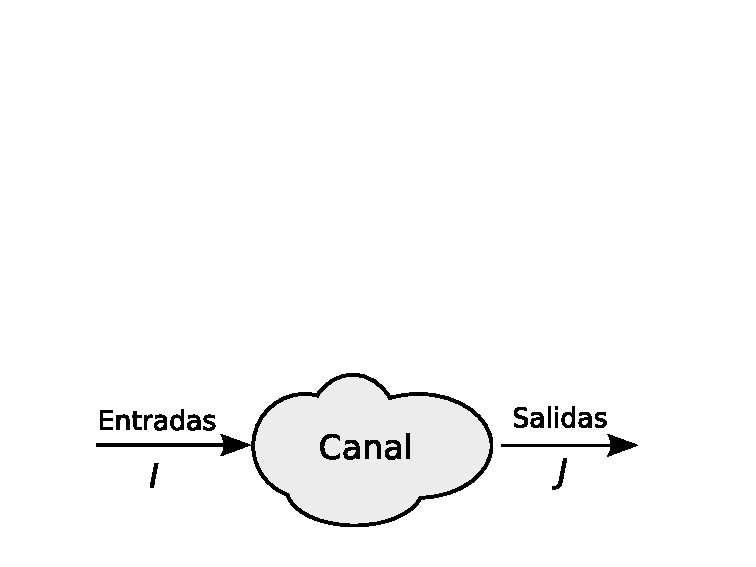
\includegraphics[scale=0.75]{canal} 
\end{center}
\caption{Representación visual de un canal}\label{fig:canal}
\end{figure}
\end{frame} 

%%%%%%%%%%%%%%%%%%%%%%%%%%%%%%%%
\begin{frame}  \small  
\begin{itemize}  


\item  Para cada $i \in I$ y $j \in J$, podemos denotar por $Pr(j|i)$ la probabilidad condicional que la salida es $j$, dado que la entrada es $i$:

\begin{center}
Pr(j $|$ i) = Pr(salida es j $|$ entrada es i).
\end{center}


\end{itemize} 

\begin{definicion}[Canales con Ruido]

Un canal $\Gamma$ con el conjunto de entrada $I$ y el conjunto de salida $J$ es una matriz cuya entrada son los Pr(j $|$ i):
\vspace{0.3cm}
\begin{center}
$\Gamma_{ij}$ = Pr(j $|$ i)	($i\in I$,$j \in J$).
\end{center}

\vspace{0.3cm}
Las entradas de $\Gamma$ están etiquetadas, por lo que el índice $i$ corresponden a las entradas, mientras que el índice $j$  corresponde a las salidas.

\vspace{0.3cm}
 Si al menos uno de los términos $\Gamma_{ij}$ con \textcolor{red}{$i\neq j$}  es distinto de \textcolor{red}{cero}, podemos decir que \textbf{\underline{el canal tiene ruido}}.
\end{definicion}
\end{frame} 

%%%%%%%%%%%%%%%%%%%%%%%%%%%%%%%%
\begin{frame}  \small  

\begin{definicion}[Canal Binario Simétrico]

Un canal binario simétrico (BSC) corresponde a un matriz de la forma

\[
\Gamma = \left( \begin{array}{lc}
            \Gamma_{00}       & \Gamma_{01}      \\
            \Gamma_{10}    & \Gamma_{11}      
           \end{array}
    \right) = \left( \begin{array}{cc}
           1-e       & e      \\
            e    & 1-e      
           \end{array}
    \right)    
\]

\end{definicion}

\begin{figure}[!hbtp]
\begin{center}
	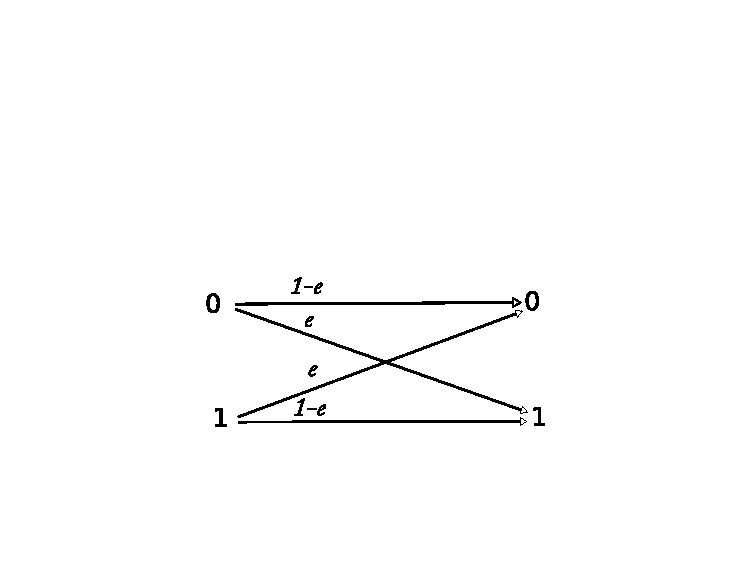
\includegraphics[scale=1]{bsc} 
\end{center}
\caption{El canal binario simétrico con probabilidad de error de bit $e$}\label{fig:bsc}
\end{figure}


\end{frame} 

%%%%%%%%%%%%%%%%%%%%%%%%%%%%%%%%



%%%%%%%%%%%%%%%%%%%%%%%%%%%%%%%%
\begin{frame}  \small  
\begin{itemize}  

\item La figura \ref{fig:bsc} es una representación de un \textcolor{red}{Canal Binario Simétrico}. 

\item  Las filas y columnas de la matriz del canal $\Gamma$ corresponden a 0 y 1, los elementos del alfabeto binario \textit{B}. 

\item El hecho que $\Gamma_{01}=\Gamma_{10}=e$ significa que los símbolos de la salida difieren de los símbolos de la entrada con una probabilidad $e$ y nos referimos como la probabilidad de error de bit. 

\item La probabilidad que un símbolo es transmitido correctamente es 
$\Gamma_{00}=\Gamma_{11}=1-e$. 

\item Usualmente asumimos que $e$ es un número pequeño positivo: por ejemplo $e=0.01$ significa que un bit de cada 100 es transmitido de forma errónea. 

\item La gravedad asociada a este porcentaje depende del escenario a estudio, ya que en algunos caso sería una tasa error inaceptable. 
\end{itemize} 

\end{frame} 

%%%%%%%%%%%%%%%%%%%%%%%%%%%%%%%%
\begin{frame}  \small 

\begin{ejemplo}

La figura \ref{fig:teclado} muestra un teclado simplificado con 6 letras A,B,C,D,E,F. Dos letras son adyacentes si un borde de una es próxima al borde de la otra. Dado dos teclas adyacentes x e y existe una probabilidad de 0.1 que cuando intento introducir la tecla $x$ pulsaré la tecla $Y$. Escribe cual es la matriz de canal para esta situación. Si intento introducir $BECA$, ¿Cual es la probabilidad que el teclado registre correctamente?\\

\end{ejemplo}

\begin{figure}[!hbtp]
\begin{center}
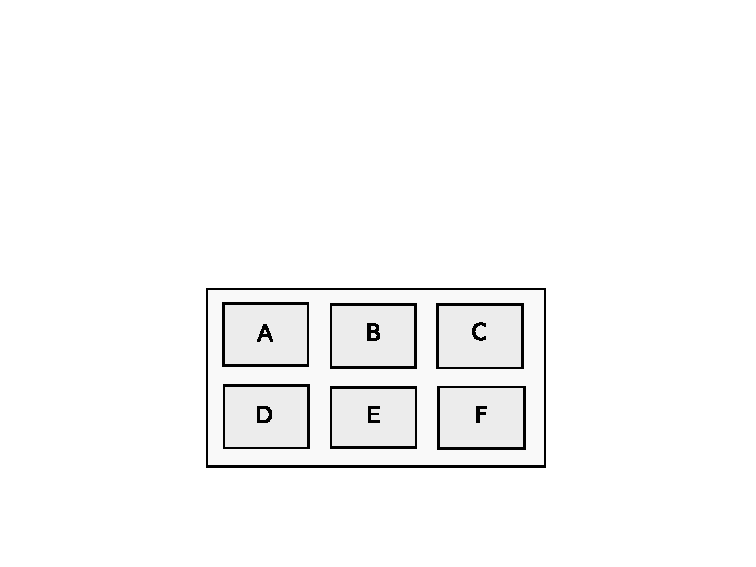
\includegraphics[scale=0.85]{teclado} 
\end{center}
\caption{Representación de un teclado simplificado}\label{fig:teclado}
\end{figure}



\end{frame} 
%%%%%%%%%%%%%%%%%%%%%%%%%%%%%%%%
\begin{frame}  \small 

\textit{\underline{Solución}}:\\
\vspace{0.5cm}
El conjunto de entrada y salida son \{A, B, C, D, E, F \}, y la matriz del canal es


\[
\Gamma = \left( \begin{array}{cccccc}
            0.8  &  0.1 & 0    & 0.1  & 0 & 0 \\
            0.1  &  0.7 & 0.1 & 0 & 0.1 &  0\\
            0     &  0.1 & 0.8 & 0 &  0 &  0.1\\
            0.1  &  0    & 0 	& 0.8 & 0.1 &  0\\
            0     &  0.1 & 0    & 0.1 & 0.7 & 0.1 \\
            0     &  0    & 0.1 & 0 & 0.1 &   0.8  
           \end{array}
    \right) 
\]

\vspace{0.5cm}
La probabilidad de introducir correctamente $BECA$ es 0.7 x 0.7 x 0.8 x 0.8 = \textbf{0.3136}.

\end{frame} 


%%%%%%%%%%%%%%%%%%%%%%%%%%%%%%%%
\begin{frame}  \small 

\begin{lema}

La suma en cada fila en una matriz de canal es igual a 1. 

\begin{center}
$\sum_{j \in J} \Gamma_{ij}$ = 1 para todo $i \in I$
\end{center}

\end{lema}

\end{frame} 

%%%%%%%%%%%%%%%%%%%%%%%%%%%%%%%%
\begin{frame}  \small 

\begin{ejercicio} 

Un canal asimétrico binario es similar a un BSC, excepto que la probabilidad de error cuando enviamos 0 es $a$, y la probabilidad de error cuando enviamos 1 es $b$, donde $a \neq b$. Establezca la matriz para este canal.
\end{ejercicio} 



\textit{\underline{Solución}}:\\

\[
\Gamma =  \left( \begin{array}{cc}
           1-a       & a      \\
            b    & 1-b      
           \end{array}
    \right)    
\]

\end{frame} 
%%%%%%%%%%%%%%%%%%%%%%%%%%%%%%%%
\begin{frame}  \small 

\begin{ejercicio} 

Un canal simétrico ternario es un  canal para el cual el conjunto de entrada $I$ y el conjunto de salida $J$ son los mismo $\{0,1,2\}$, y la probabilidad que un símbolo $i$ sea $j \neq i$ es $x$. Establezca la matriz para este canal.

\end{ejercicio} 


\textit{\underline{Solución}}:\\

\[
\Gamma =  \left( \begin{array}{ccc}
           1-2x       & x  & x    \\
            x       &  1-2x  & x    \\
           x       & x  & 1-2x    \\
           \end{array}
    \right)    
\]

\end{frame} 

\subsection{Transmitir una fuente mediante un canal}

%%%%%%%%%%%%%%%%%%%%%%%%%%%%%%%%
\begin{frame}   \footnotesize
{
\setbeamercolor{block title}{bg=blue!40!black, fg=white}
\setbeamercolor{block body}{bg=white!05, fg=black}
\begin{block}{Sección 5.1.1}
Transmitir una fuente mediante un canal
\end{block}
}
\end{frame} 


%%%%%%%%%%%%%%%%%%%%%%%%%%%%%%%%
\begin{frame} \frametitle{Transmitir una fuente mediante un canal} \small  
\begin{itemize}  

\item Supóngase que un símbolo $i$ en el conjunto de entrada $I$ ocurre con probabilidad $p_i$, por lo que tenemos una distribución de probabilidad p en $I$.

\item Podemos pensar que la entrada de un canal $\Gamma$ es generada por una fuente (I,p). 

\item Similarmente, estableciendo $q_j$ la probabilidad que el símbolo de salida es $j$, la salida puede ser considerada como una fuente $(J,q)$.
 
\item  El siguiente teorema describe la relación entre $p$ y $q$. 


\end{itemize} 

\begin{teorema}
Sea $\Gamma$ una matriz de canal, y sea las distribuciones asociadas con la fuente de entrada (I,p) y la fuente de salida (J,q) escrita como vectores,

\begin{center}
$p = [p_1,p_2,\ldots,p_m]$,	$q = [q_1,q_2,\ldots,q_n]$, entonces: $q = p\Gamma$.
\end{center}

\end{teorema}


\end{frame} 



%%%%%%%%%%%%%%%%%%%%%%%%%%%%%%%%
\begin{frame}  \small  

\begin{itemize}  

\item Ahora entonces tenemos un modelo en el cual el \textcolor{red}{canal $\Gamma$} puede ser considerado como un enlace entre dos fuentes, $(I,p)$ y $(J,q)$.
\item  La primera fuente es producida por el Emisor, mientras que la segunda fuente, el resultado de la transmisión mediante $\Gamma$, está disponible al Receptor.  
\item Estas fuentes están relacionadas por la ecuación \textcolor{red}{$q=p\Gamma$}.
\end{itemize} 

\end{frame} 



%%%%%%%%%%%%%%%%%%%%%%%%%%%%%%%%
\begin{frame}  \small 

\begin{ejemplo}\label{ej:BSC}

Establezca las ecuaciones que vinculan $p = [p_0,p_1]$ y $q = [q_0,q_1]$ cuando $\Gamma$ es el BSC con probabilidad de error de bit $e$. 
Si $e = 0.1$ y $p = [0.7, 0.3]$, ¿Cual es el valor de q?.\\

\end{ejemplo}

\textit{\underline{Solución}}:\\
\vspace{0.3cm}
La ecuación de la matriz es:

\[
\left( \begin{array}{lc}
            q_{0}       & q_{1}      \\
           \end{array}
    \right)  = \left( \begin{array}{lc}
            p_{0}       & p_{1}      \\
           \end{array}
    \right) \left( \begin{array}{cc}
           1-e       & e      \\
            e    & 1-e      
           \end{array}
    \right)    
\]

la cual es equivalente a las ecuaciones:

\begin{center}
$q_0	= p_0 \times (1 - e) + p_1 \times  e$\\
$q_1	= p_0 \times e  + p_1 \times  (1 - e)$
\end{center}

Si $e = 0.1$ y $p = [0.7, 0.3]$ entonces $q = [0.66, 0.34]$


\end{frame} 


%%%%%%%%%%%%%%%%%%%%%%%%%%%%%%%%
%%%%%%%%%%%%%%%%%%%%%%%%%%%%%%%%
%EJERCICIO %%%%%%%%%%%%%%%%%%%%%%%%%%%%%%%
%%%%%%%%%%%%%%%%%%%%%%%%%%%%%%%%


%%%%%%%%%%%%%%%%%%%%%%%%%%%%%%%%
\begin{frame}  \small \begin{ejercicio} 

Supongase que las salidas de un canal $\Gamma_1$ son las símbolos de entrada para un canal $\Gamma_2$, y $\Gamma$ es el resultado del canal combinado. En esta situación diremos que $\Gamma$ es el resultado de combinar $\Gamma_1$ y $\Gamma_2$ en series. ¿Cual es la relación entre las matrices  $\Gamma_1$ y $\Gamma_2$ y  $\Gamma$ ?
\end{ejercicio}

\textit{\underline{Solución}}:\\
\vspace{0.5cm}
Sea p la entrada a $\Gamma_1$, q la salida de $\Gamma_1$  y la entrada a $\Gamma_2$, $r$ la salida de $\Gamma_2$.\\
\vspace{0.3cm}
Entonces  r = q $\times \Gamma_2$  = p $\times \Gamma_1$ $ \times \Gamma_2$.\\
\vspace{0.3cm}
Por tanto $\Gamma$ es la matriz producto de $\Gamma_1 \times \Gamma_2$.

\end{frame} 


%%%%%%%%%%%%%%%%%%%%%%%%%%%%%%%%
\begin{frame}  \small 

\begin{ejercicio} \label{ej:5.6}

Considere el canal simétrico binario con probabilidad de error por bit $e = 0.01$. Si la entrada tiene una distribución de probabilidad p = [0.6, 0.4]. ¿Cual es la distribución de probabilidad q?. \\
Compare las entropías de la entrada y salida.
\end{ejercicio}
\textit{\underline{Solución}}:\\

\[
\left( \begin{array}{lc}
            q_{0}       & q_{1}      \\
           \end{array}
    \right)  = \left( \begin{array}{lc}
            p_{0}       & p_{1}      \\
           \end{array}
    \right) \left( \begin{array}{cc}
           1-0.01       & 0.01      \\
            0.01    & 1-0.01      
           \end{array}
    \right)    
\]
\begin{center}
$q_0	= p_0 \times (1 - e) + p_1 \times e$  = $0.6 \times 0.99 + 0.4 \times 0.01=0.598$ \\
$q_1	= p_0 \times e  + p_1 \times (1 - e)$ = $0.6 \times 0.01 + 0.4 \times 0.99=0.402$
\end{center}

\begin{center}
$H(p) = H([0.6,0.4])	\approx  0.9709$;  $H(q) = H([0.598,0.402])	\approx  0.9721$
\end{center}

\textbf{La incertidumbre ha crecido a la hora de transmitir por un canal con ruido}.
\end{frame} 

%%%%%%%%%%%%%%%%%%%%%%%%%%%%%%%%
%%%%%%%%%%%%%%%%%%%%%%%%%%%%%%%%
%SECCION %%%%%%%%%%%%%%%%%%%%%%%%%%%%%%%
%%%%%%%%%%%%%%%%%%%%%%%%%%%%%%%%


\subsection{Entropía Condicional}

%%%%%%%%%%%%%%%%%%%%%%%%%%%%%%%%
\begin{frame}   \footnotesize
{
\setbeamercolor{block title}{bg=blue!40!black, fg=white}
\setbeamercolor{block body}{bg=white!05, fg=black}
\begin{block}{Sección 5.1.2}
Entropía Condicional
\end{block}
}
\end{frame} 



%%%%%%%%%%%%%%%%%%%%%%%%%%%%%%%%
\begin{frame}  \frametitle{Entropía Condicional}\small  
\begin{itemize}  

\item La \textbf{existencia de errores} tiende a equiparar las probabilidades, ya que los \textcolor{red}{símbolos que ocurren con más frecuencia son transmitidos erróneamente más a menudo}.

\item   En el ejemplo \ref{ej:BSC} la incertidumbre de la entrada y la salida son, respectivamente,

\begin{center}
$h(0.7) \approx 0.881,	h(0.66) \approx 0.925$,
\end{center}

\item \textcolor{red}{La incertidumbre es incrementada por la transmisión a través de un canal con ruido}. 

\item Un problema más sutil es describir la situación desde el \textbf{punto de vista del Receptor}, para aquellos los cuales la salida es la única información disponible sobre la entrada.

\begin{center}
¿Cuanta información sobre la \textbf{entrada} está disponible al Receptor que conoce la salida de $\Gamma$?
\end{center}
\end{itemize} 
\end{frame}
%%%%%%%%%%%%%%%%%%%%%%%%%%%%%%%%
\begin{frame} [fragile] \small  
\begin{itemize}  
\item Estableceremos el modelo en términos de una entrada que es enviada a través de un canal para producir una salida.

\item  Una distribución de probabilidad $t$ en el conjunto $I \times J$:

\begin{center}
$t_{ij}$ = Pr(entrada es $i$ y salida es $j$). \\
$t_{ij}$ =  Pr(salida es $j$ $|$ entrada es $i$) $\times$ Pr(entrada es $i$) = $\Gamma_{ij} p_i$
\end{center}

\item Teniendo $t$, todas las otras cantidades pueden ser derivadas a través de $t$ utilizando las ecuaciones

\begin{center}
$p_i=\sum_j t_{ij} \;\;$  $q_j=\sum_i t_{ij}$ \;\; $\Gamma_{ij}=t_{ij}/p_i$
\end{center}

%\item Concretamente, $p$ y $q$ son las distribuciones marginales asociadas con $t$.
\end{itemize} 
\vspace{0.3cm}
\begin{center}
        Fuente X  $\rightarrow$ Canal $\Gamma$   $\rightarrow$  Salida Y\\
      $p_i$   \,\,\, \,\,\, \,\,\,    $t_{ij}$     \,\,\, \,\,\,\,\,\,  $q_j$    
\end{center}




\end{frame} 
%%%%%%%%%%%%%%%%%%%%%%%%%%%%%%%%
\begin{frame}  \small 

\begin{ejemplo}

Sea $\Gamma$ el BSC con una probabilidad de bit de error  e = 0.1, y sea la distribución de la fuente p = [0.7, 0.3]. Calcular t.
\end{ejemplo}


\textit{\underline{Solución}}:\\
\vspace{0.15cm}

\footnotesize

\[
 t = p \times \Gamma = (0.7 \; 0.3) \times 
     \left( \begin{array}{cc}
           0.9       & 0.1     \\
            0.1    & 0.9      
           \end{array}
    \right) =
     \left( \begin{array}{cc}
            0.63     & 0.07     \\
            0.03    & 0.27      
           \end{array}
    \right)
\]

\begin{table}[h!]\footnotesize
    \centering
    \begin{tabular}{cccc}\hline\hline
\textbf{X (entrada)} & \textbf{Y (salida)}  & \textbf{Prob. conjunta p(x,y)} & \textbf{Explicación}\\\hline\hline
0 & 0 & 0.7 $\times$ (1-e) = 0,7 $\times$ 0,9 = 0.63   & 0 enviado correctamente \\
0 & 1 & 0.7 $\times$ e = 0.07 & 0 se corrompe \\
1 & 0 & 0.3 $\times$ e = 0.03 & 1 se corrompe \\
1 & 1 & 0.3 $\times$ (1-e) = 0.27 & 1 enviado correctamente\\\hline\hline
\textbf{TOTAL} & & 0.63+0.07+0.03+0.27 = 1 & 
    \end{tabular}

\end{table}


\end{frame} 
%%%%%%%%%%%%%%%%%%%%%%%%%%%%%%%%
\begin{frame}  \small 

\begin{ejemplo}

Sea $\Gamma$ el BSC con una probabilidad de bit de error  e = 0.1, y sea la distribución de la fuente p = [0.7, 0.3]. Calcular q.
\end{ejemplo}


\textit{\underline{Solución}}:\\
\vspace{0.3cm}

\begin{enumerate} \footnotesize
    \item \[
\Gamma =  \left( \begin{array}{cc}
           1-e       & e      \\
            e    & 1-e      
           \end{array}
    \right) =  \left( \begin{array}{cc}
           0.9       & 0.1     \\
            0.1    & 0.9      
           \end{array}
    \right) 
\]


\[
\left( \begin{array}{lc}
            q_{0}       & q_{1}      \\
           \end{array}
    \right)  = \left( \begin{array}{lc}
            0.7       & 0.3      \\
           \end{array}
    \right) \left( \begin{array}{cc}
            0.9       & 0.1      \\
            0.1    & 0.9      
           \end{array}
    \right)    = (0,66 \; 0.34)
\]

\begin{center}
$q_0	 = 0.7 \times 0.9 + 0.3 \times 0.1=0.66$ \\
$q_1	 = 0.7 \times 0.1 + 0.3 \times 0.9=0.34$
\end{center}


 \item 

 \[
 t = p \times \Gamma = (0.7 \; 0.3) \times 
     \left( \begin{array}{cc}
           0.9       & 0.1     \\
            0.1    & 0.9      
           \end{array}
    \right) =
     \left( \begin{array}{cc}
            0.63     & 0.07     \\
            0.03    & 0.27      
           \end{array}
    \right)
\]

\begin{center}
$q_0	 = 0,63 + 0,03 =0.66$ \\
$q_1	 = 0,07 + 0.27 =0.34$
\end{center}

\end{enumerate}

\vspace{0.3cm}

\end{frame} 



%%%%%%%%%%%%%%%%%%%%%%%%%%%%%%%%
\begin{frame}  \small 


\begin{definicion} [Entropía Condicional]

Con las anotaciones anteriores, la entropía condicional H(p $|$ q) es definida por 

\begin{center}
H(p $|$ q) = H(t) - H(q).
\end{center}
\end{definicion}

\begin{itemize}
\item  La motivación es que \textcolor{red}{H(t)} mide la incertidumbre sobre el \textcolor{red}{par entrada-salida (i,j)} y \textcolor{blue}{H(q)} mide la incertidumbre sobre la \textcolor{blue}{salida $j$}. 

\item  Restando la segunda cantidad, \textcolor{blue}{H(q)}, de la primera, \textcolor{red}{H(t)}, representa la incertidumbre de un \textbf{Receptor que conoce la salida y está intentando determinar la entrada}.

\begin{itemize}\footnotesize
\item  Debido a que las distribuciones de entrada y salida están vinculadas por la ecuación $q=p\Gamma$, por lo que $H(p|q)$ solo depende de $\Gamma$ y $p$. 

\item  Usualmente nos referimos a esta cantidad como entropía condicional de $p$ con respecto la transmisión a través de $\Gamma$ y viene denotado por $H(\Gamma;p)$ : $H(\Gamma;p) = H(p|q)$ (donde $q=p\Gamma$) 
 \end{itemize}
\end{itemize}

\textcolor{red}{Mide cuánta incertidumbre queda en la salida después de conocer lo que se envió.}

\begin{itemize}\tiny
    \item Si el canal fuera perfecto (sin ruido), entonces H(p$|$q)=0. Al conocer q, conoces exactamente p.
    \item Si el canal fuera totalmente aleatorio (e=0.5), entonces H(p$|$q)=H(p). Saber q no aporta ninguna información sobre p.
\end{itemize}

\end{frame} 


%%%%%%%%%%%%%%%%%%%%%%%%%%%%%%%%
\begin{frame}  \small 

\begin{ejemplo}

Sea $\Gamma$ el BSC con una probabilidad de bit de error  e = 0.1, y sea la distribución de la fuente p = [0.7, 0.3]. Calcular $H (\Gamma ; p)$.\\

\end{ejemplo}


\textit{\underline{Solución}}:\\
\vspace{0.5cm}
Ya que $t_{ij} = p_i \Gamma_{ij}$ 

\[
\Gamma =  \left( \begin{array}{cc}
           1-e       & e      \\
            e    & 1-e      
           \end{array}
    \right) =  \left( \begin{array}{cc}
           0.9       & 0.1     \\
            0.1    & 0.9      
           \end{array}
    \right) ;
\]

\[
 t = \Gamma \times p = 
     \left( \begin{array}{cc}
           0.9       & 0.1     \\
            0.1    & 0.9      
           \end{array}
    \right) \times (0.7 \; 0.3) \  = 
     \left( \begin{array}{cc}
            0.63     & 0.07     \\
            0.03    & 0.27      
           \end{array}
    \right)
\]
\vspace{0.3cm}

$H(t) = 0.63 \times log_2(1/0.63)+ 0.07 \times log_2(1/0.07) + 0.03 \times log_2(1/0.03)$ $ + 0.27 \times log_2(1/0.27)$ $\approx 1.350$
\vspace{0.3cm}

Ya que $q_j = \sum_i t_{ij}$ tenemos que q = [0.66,0.34] y $H(q) \approx 0.925$. 

\vspace{0.2cm}
Por tanto, 
\begin{center}
$H (\Gamma ; p) = H (t) - H (q) \approx 1.350 - 0.925 = 0.425.$
\end{center}




\end{frame} 

%%%%%%%%%%%%%%%%%%%%%%%%%%%%%%%%
\begin{frame}  \small 

El resultado general para un \textcolor{red}{\textbf{canal simétrico binario}} es como sigue:
\begin{teorema}\label{teorema:entropia}

Sea $\Gamma$ el BSC con una probabilidad de bit error $e$, y sea $p$ la distribución de la fuente $[p_0,p_1] = [p, 1-p]$. Entonces

\begin{center}
$H(\Gamma ;p) = h(p)+ h (e)- h (q), $
\end{center}
donde 
\begin{center}
$q = p \times (1 - e) + (1 - p) \times e$, 
\end{center}
y $h$ es la función de entropía estándar definida como\\
\begin{center}
    $h(x) = x \times log_2(1/x) + (1 - x)\times log_2(1/(1 - x))$.
\end{center}
\end{teorema}

\begin{itemize}\tiny
     \item  \textcolor{red}{\textbf{h(p)}} mide la incertidumbre de la fuente de entrada (cuán balanceados están los símbolos 0 y 1).
     \item  \textcolor{red}{\textbf{h(e)}} mide la incertidumbre introducida por el canal (ruido).
     \item  \textcolor{red}{\textbf{h(q)}} mide la incertidumbre total de la salida Y, combinando el efecto del ruido y la distribución original.
\end{itemize}

\end{frame} 


%%%%%%%%%%%%%%%%%%%%%%%%%%%%%%%%
\begin{frame}  \small 

\begin{ejemplo} 
En el caso uniforme  p=0.5:
BSC con probabilidad de error e:
\begin{center}
$P(Y=X) = 1-e\;\;\;$,  P($Y \neq X$)=e    



    \begin{center}
    $q= 0.5 \times (1-e)+0.5 \times e=0.5$
    \end{center}

\end{center}

\end{ejemplo}

\textit{\underline{Solución}}:\\

\begin{itemize}
    \item Esto significa que cada símbolo transmitido tiene exactamente la misma probabilidad de confundirse.
    \item  No hay símbolo privilegiado: el canal trata a ``0'' y ``1'' por igual.

    \item Con lo cual 
    
    \begin{center}
    $H(\Gamma ;p) = h(p)+ h (e)- h (q)  $\\
    \vspace{0.3cm}
    $H(\Gamma ;p) = h(0.5)+ h (e)- h (0.5) = h(e) $
    \end{center}
    
\end{itemize}
\end{frame} 

%%%%%%%%%%%%%%%%%%%%%%%%%%%%%%%%
%%%%%%%%%%%%%%%%%%%%%%%%%%%%%%%%
%EJERCICIOS %%%%%%%%%%%%%%%%%%%%%%%%%%%%%%%
%%%%%%%%%%%%%%%%%%%%%%%%%%%%%%%%

%%%%%%%%%%%%%%%%%%%%%%%%%%%%%%%%
\begin{frame}  \small 

\begin{ejercicio} 

Considere el canal simétrico binario con probabilidad de error por bit $e = 0.01$. (Ejercicio  \ref{ej:5.6}). Si la entrada tiene una distribución de probabilidad p = [0.6, 0.4]. Calcule la distribución $t$ y la entropía condicional $H(\Gamma;p)$. Verifica que la respuesta del ejercicio anterior cumple la formula del Teorema \ref{teorema:entropia}.

\end{ejercicio}

\textit{\underline{Solución}}:\\
\[
\Gamma =  \left( \begin{array}{cc}
           1-e       & e      \\
            e    & 1-e      
           \end{array}
    \right) =  \left( \begin{array}{cc}
           0.99       & 0.01     \\
            0.01    & 0.99    
           \end{array}
      \right)      
\]   
\[
     t =    \left( \begin{array}{cc}
           0.99       & 0.01     \\
            0.01    & 0.99    
           \end{array}       
    \right) 
    \times (0.6\; 0.4)
     = \left( \begin{array}{cc}
            0.594     & 0.006     \\
            0.004    & 0.396      
           \end{array}
    \right)
\]


$H(t) \approx 1.0517$ y $q_j = \sum_i t_{ij}$ tenemos que q = [0.598,0.402], y 
$H(q) \approx 0.9721$. 


\begin{center}
$H (\Gamma ; p) = H (t) - H (q) \approx 1.0517 - 0.9721 \approx  0.0796.$
\end{center}

\textbf{Verifico el Teorema \ref{teorema:entropia}.}

\begin{center}
 $H(\Gamma ;p) = h(p)+h(e)-h(q) = 0.9709 + 0.0807 - 0.9721 \approx 0,0795$
\end{center}
Ya que: $ h(e) = h(0.01) = 0.01 \times log_2(1/0.01) + 0.99 \times log_2(1/0.99) =0.0807 $


\end{frame} 

%%%%%%%%%%%%%%%%%%%%%%%%%%%%%%%%

%%%%%%%%%%%%%%%%%%%%%%%%%%%%%%%%
%%%%%%%%%%%%%%%%%%%%%%%%%%%%%%%%
%SECCION %%%%%%%%%%%%%%%%%%%%%%%%%%%%%%%
%%%%%%%%%%%%%%%%%%%%%%%%%%%%%%%%


\subsection{La capacidad de un canal}


\begin{frame}   \footnotesize
{
\setbeamercolor{block title}{bg=blue!40!black, fg=white}
\setbeamercolor{block body}{bg=white!05, fg=black}
\begin{block}{Sección 5.1.3}
La capacidad de un canal
\end{block}
}
\end{frame} 


%%%%%%%%%%%%%%%%%%%%%%%%%%%%%%%%
\begin{frame}  \frametitle{La capacidad de un canal}\small  
\begin{itemize}  

\item El número máximo de bits de \textbf{información útil} que se pueden transmitir por el canal, si diseñamos un código de transmisión óptimo.

%\item Cuántos bits “reales” puedes transmitir por símbolo, incluso aunque haya errores, si usas un código de corrección de errores ideal.


\item Haciendo uso de las definiciones que hemos realizado previamente, estableceremos la definición de la \textbf{capacidad de un canal}.


\begin{itemize}
\item $H(p)$: La \textbf{incertidumbre} sobre los símbolos emitidos por una \textbf{fuente de entrada p};
\item $H (\Gamma ; p)$:  La \textbf{incertidumbre} sobre los símbolos emitidos por $p$ desde el punto de vista del \textbf{Receptor} quien conoce los símbolos de \textbf{salida emitidos} por la fuente $q=p\Gamma$.
\end{itemize}

\end{itemize} 


\vspace{0.3cm}
\begin{teorema}

Sea $\Gamma$ un canal y $p$ una distribución de entrada para $\Gamma$. Entonces

 \begin{center}
$H(\Gamma ;p) \leq H(p).$
\end{center}

La igualdad la obtenemos sii p y $q = p\Gamma$ son distribuciones independientes.

\end{teorema}

\end{frame} 

%%%%%%%%%%%%%%%%%%%%%%%%%%%%%%%%
\begin{frame} {Función de información mutua, $f_{\Gamma}(p)$} \small  
\begin{itemize}  


%\item  Ya que $f_{\Gamma}(p)$ es la diferencia entre dos medidas de incertidumbre, podemos pensar que es una medida de información. 


\item $f_{\Gamma}(p)$ representa la información sobre los \textbf{símbolos} emitidos por la \textbf{fuente de entrada} que está disponible al \textbf{Receptor} que conoce los \textbf{símbolos} emitidos por la \textbf{fuente de salida}. 

\begin{center}
$f_{\Gamma}(p) = H(p)-H(\Gamma ;p).$
\end{center}

\item Por ejemplo, supongamos que $\Gamma$ es el BSC con una probabilidad de error de bit e=0.1 y la distribución de entrada es $p = [0.7,0.3]$. Anteriormente hemos calculado que $H(p) = h(0.7) \approx 0.881$ y $H(\Gamma;p) \approx 0.425$, por lo que:

\begin{center}
$f_{\Gamma}(p) = H(p)-H(\Gamma ;p) \approx 0.881 - 0.425 = 0.456$
\end{center}

\end{itemize} 

\begin{definicion}[Capacidad]

La capacidad $\gamma$ de $\Gamma$ es máximo valor de $f_{\Gamma}(p)$, tomado del conjunto $\mathrm{P}$ de todas las distribuciones de probabilidad en un conjunto de tamaño m (el número de filas de $\Gamma$).

\begin{center}
$\gamma = 	max f_{\Gamma}(p) = max ( H(p)-H(\Gamma ;p))$
\end{center}

\end{definicion}

\end{frame} 


%%%%%%%%%%%%%%%%%%%%%%%%%%%%%%%%
%\begin{frame}  \small  
%\begin{itemize}  

%\item Supongase que dado un canal $\Gamma$ que acepta un alfabeto de entrada $I$  de tamaño m, o que la matriz del canal tiene m filas, entonces para cada  distribución de probabilidad $p$ sobre $I$ tendremos un valor de $f_{\Gamma}(p)$.


%\end{itemize} 
%\begin{definicion}[Capacidad]

%La capacidad $\gamma$ de $\Gamma$ es máximo valor de $f_{\Gamma}(p)$, tomado del conjunto $\mathrm{P}$ de todas las distribuciones de probabilidad en un conjunto de tamaño m (el número de filas de $\Gamma$).

%\begin{center}
%$\gamma = 	max f_{\Gamma}(p) = max ( H(p)-H(\Gamma ;p))$
%\end{center}

%\end{definicion}
%\end{frame} 

%%%%%%%%%%%%%%%%%%%%%%%%%%%%%%%%
%%%%%%%%%%%%%%%%%%%%%%%%%%%%%%%%
%EJERCICIOS %%%%%%%%%%%%%%%%%%%%%%%%%%%%%%%
%%%%%%%%%%%%%%%%%%%%%%%%%%%%%%%%

%TODO

%%%%%%%%%%%%%%%%%%%%%%%%%%%%%%%%
%\begin{frame}  \small \begin{ejercicio} \end{ejercicio}\end{frame} 
%%%%%%%%%%%%%%%%%%%%%%%%%%%%%%%%

%%%%%%%%%%%%%%%%%%%%%%%%%%%%%%%%
\begin{frame}  \small  


\begin{teorema}
La \textcolor{red}{capacidad del BSC} con probabilidad de error de bit $e$  $(0 \leq e \leq 0.5 )$ es

\begin{center}
$\gamma = 1-h(e)$,
\end{center}

donde $h(e) = e \times log_2(1/e) + (1 - e) \times  log_2 (1/(1 - e)).$
\end{teorema}
\begin{itemize}  
\item  En la mayoría de las situaciones reales, $e$ es pequeño, por lo que el valor de $h(e)$ es cercano a 0 y $\gamma$ a 1.


\item La capacidad del canal con el valor de e:
\begin{itemize}  

\item  e = 0.01 es 

\begin{center}
$\gamma = 1 - h(0.01)	= 1 - 0.01 \times  log_2(1/0.01) - 0.99 \times log_2(1/0.99) = 0.919$.
\end{center}

\item  e = 0.5 es 

\begin{center}
$\gamma = 1 - h(0.5)	= 1 - 0.5 \times  log_2(1/0.5) - 0.5 \times log_2(1/0.5) = 0$.
\end{center}
\end{itemize}
\end{itemize}

\textcolor{red}{Cuando el canal tiene una probabilidad de error (e) de 0.5, es completamente ruidoso y no se transmite información, por tanto, la capacidad del canal es 0 bits por símbolo.}
\end{frame} 

%%%%%%%%%%%%%%%%%%%%%%%%%%%%%%%%
\begin{frame}  \small  


En resumen, si por ejemplo e = 0.2:

\begin{center}
$\gamma = 1 - h(0.2)	= 1 - 0.2 \times  log_2(1/0.2) - 0.8 \times log_2(1/0.8) = 1 - 0.7219 = 0.2781$.
\end{center}


Esto significa:

\begin{itemize}
    \item Por cada 1 bit transmitido, solo 0.278 bits pueden ser ``información útil pura''. Los otros 0.722 bits tienen que ser redundancia o protección si quieres comunicación sin errores.
    \item Por tanto, de cada 100 bits que envías, 27.8 pueden ser información, y 72.2 deben ser redundancia para corregir el ruido.
\end{itemize}


\begin{table}
    \centering
    \begin{tabular}{ccc}
         \textbf{Concepto} & \textbf{Valor} & \textbf{Interpretación} \\\hline\hline
         e & 0.2 & 20 \% de errores en el canal\\
         h(e) & 0.7219 & Ruido del canal\\
         $\gamma =1 - h(e)$ &  0.2781 & Máx. proporción de bits útiles\\
    \end{tabular}
\end{table}

\textbf{Significado}: Solo puedes usar el 27.8 \% de la capacidad para información; el resto debe usarse para redundancia.

\end{frame} 

%%%%%%%%%%%%%%%%%%%%%%%%%%%%%%%%
%%%%%%%%%%%%%%%%%%%%%%%%%%%%%%%%
\begin{frame}[fragile]  {bsc\_demo.py}\footnotesize  

\tiny
\begin{verbatim}  
python3 bsc_demo.py ABACAB --error 0.2 --seed 111
python3 bsc_demo.py ABACABAAABABABABABBBBCBCCCCCCCBBBBABABABABCBBBABABAB --error 0.2 --seed 111
python3 bsc_demo.py ABACABABBBABABABABBBCBCBBBBABBCBCBCBBBABABABBABABABABABABABABA --error 0.2 --seed 111
\end{verbatim}

\begin{verbatim}  
== Parametros ==
Mensaje: ABACAB | e(BSC)=0.200 | seed=111

== Codificacion ==
Mapa: A->00, B->01, C->10 ('11' → '?')
X bits (12): 000100100001
Y bits (12): 000100010001
Bit flips observados: 2/12 (~0.1667)

Entrada decodificada : ABACAB
Salida decodificada  : ABABAB
Errores de símbolo   : 1/6 (~0.1667)

== Matriz del canal estimada M'(condicional Y|X) ==
conteos: [[   8,    1], 
          [   1,    2]]   (X=0:9, X=1:3)
M'= [[0.8889, 0.1111], 
     [0.3333, 0.6667]]

Matriz BSC teorica con e parametro:
M  = [[0.8000, 0.2000], 
      [0.2000, 0.8000]]

El error total observado es aproximadamente 0.1667 vs e parametro 0.2000
\end{verbatim}

\end{frame} 
%%%%%%%%%%%%%%%%%%%%%%%%%%%%%%%%
%%%%%%%%%%%%%%%%%%%%%%%%%%%%%%%%
\begin{frame}[fragile]  {bsc\_demo.py}\footnotesize  

\tiny
\begin{verbatim}  
== Entropias empiricas (bits) ==
H(X) o H(p)  = 0.8113
    == Detalle del calculo de H(000100100001) ==
    x   freq     p(x)    log2(1/p)    p*log2(1/p)
    0      9   0.7500       0.4150         0.3113
    1      3   0.2500       2.0000         0.5000
                          TOTAL ->         0.8113
H(Y)  o H(q) = 0.8113
    == Detalle del calculo de H(000100010001) ==
    x   freq     p(x)    log2(1/p)    p*log2(1/p)
    0      9   0.7500       0.4150         0.3113
    1      3   0.2500       2.0000         0.5000
                          TOTAL ->         0.8113
                          
Incertidumbre total del sistema completo (entrada + salida).
H(X,Y) o H(t).   = 1.4183

Si ya conozco la salida del canal Y, ¿cuánta duda me queda sobre cuál fue la entrada X?.
H(Y|X) o H(p|q) o H(G;p)  = 0.6070

Informacion mutua entre entrada y salida del canal.
fG(p)  = 0.2043

==  Teoria BSC ==
p=(0.7500,0.2500)  e=0.2000  q=(0.6500,0.3500)

h(p)=H(X)=0.8113   h(e)=0.7219   h(q)=H(Y)=0.9341

H(G;p)=h(p)+h(e)-h(q) = 0.5991       fG(p)= H(p)-H(G;p)= 0.2121

Capacidad = 1 - h(e) = 0.2781 bits/canal

I_emp=0.2043  --> No excede la capacidad del canal

\end{verbatim}

\end{frame} 
%%%%%%%%%%%%%%%%%%%%%%%%%%%%%%%%
\begin{frame}[fragile]  {bsc\_demo.py}\footnotesize  

\begin{center}
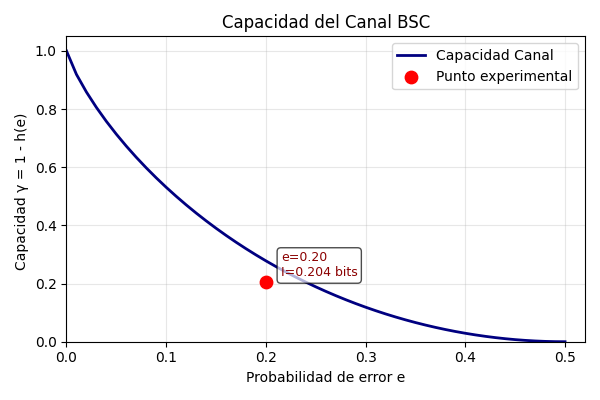
\includegraphics[scale=0.7]{capacidadCanal.png}
\end{center} 

\end{frame} 

%%%%%%%%%%%%%%%%%%%%%%%%%%%%%%%%
%%%%%%%%%%%%%%%%%%%%%%%%%%%%%%%%
%SECCION %%%%%%%%%%%%%%%%%%%%%%%%%%%%%%%
%%%%%%%%%%%%%%%%%%%%%%%%%%%%%%%%

 
\section{Comunicación utilizando un canal con ruido}

\begin{frame}   \footnotesize
{
\setbeamercolor{block title}{bg=blue!60!black, fg=white}
\setbeamercolor{block body}{bg=blue!10, fg=black}
\begin{block}{Sección 2}
Comunicación utilizando un canal con ruido
\end{block}
}
\end{frame} 
%%%%%%%%%%%%%%%%%%%%%%%%%%%%%%%%
\begin{frame}  \frametitle{Comunicación utilizando un canal con ruido}\small  
\begin{itemize} 

 \item Vamos a centrarnos en la transmisión de los mensajes codificados a través de un canal con ruido, en el caso concreto de mensajes codificados en el \textcolor{red}{alfabeto binario} $\mathbb{B} =\{0,1\}$, transmitidos mediante un \textcolor{red}{canal binario simétrico}.

\item  La fuente emite una cadena de símbolos que son codificados como palabras binarias, todas con la \textbf{misma longitud} $n$ donde $n$ será escogido por alguna condición deseable. 


\item Por ejemplo, supongase que la fuente es un control remoto que guía un robot a través de una red de calles, desde Norte-Sur a Este-Oeste. Algunas calles presentan obstáculos y algunas de ellas son de una sola dirección. 

\item Para mover el robot de un punto a otro, el controlador debe enviar una secuencia de símbolos N, S, E, O, según corresponda.

\item En este caso el alfabeto es X = \{N, S, E, O\}. Tomando n = 2, un código apropiado $c: X \rightarrow\mathbb{B}^{2}$ podría ser:

\begin{center}
$N \mapsto 00, S \mapsto 01, E \mapsto 10, O \mapsto 11$
\end{center}


\end{itemize} \end{frame} 
%%%%%%%%%%%%%%%%%%%%%%%%%%%%%%%%

\begin{frame}  \frametitle{Comunicación utilizando un canal con ruido}\small  
\begin{itemize} 

\item  Utilizando este código la secuencia de instrucciones mostrada en la figura \ref{fig:robot} es codificada como sigue:

\begin{center}
$(E, N, N, E, S, E, E, S, O)	\mapsto	100000100110100111$
\end{center}

\begin{figure}[!hbtp]
\begin{center}
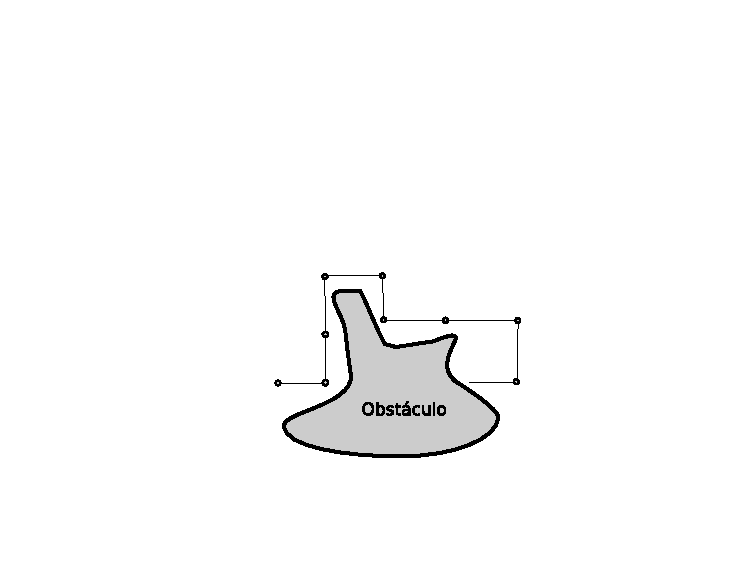
\includegraphics[scale=1]{robot} 
\end{center}
\caption{La ruta E,N,N,E,S,E,E,S,O}\label{fig:robot}
\end{figure}

\end{itemize} \end{frame} 

%%%%%%%%%%%%%%%%%%%%%%%%%%%%%%%%
\begin{frame}  \small  
\begin{itemize} 

\item El valor n=2 es claramente el menor valor posible para un código binario para cuatro mensajes.
 
\item  Sin embargo, este código tiene una \textcolor{red}{desventaja} que si cualquier error ocurre en los bits que son transmitidos, el robot no será capaz de detectarlo. 
 
\item Por ejemplo, supongamos que 
\begin{enumerate}
    \item el símbolo que queremos transmitir es $S$, por lo que $01$ es \textbf{enviado}, 
    \item  si el primer bit es \textcolor{red}{alterado en la transmisión}, 
    \item por lo que 11 es recibido. 
    \item El robot decodificará como $O$, y no tiene capacidad de conocer que un error ha sucedido.

\end{enumerate}


\end{itemize} \end{frame} 

%%%%%%%%%%%%%%%%%%%%%%%%%%%%%%%%
\begin{frame}  \footnotesize  
\begin{itemize} 

\item Los mensajes originados de alguna fuente y son expresados en un alfabeto $X$. Nos referimos a la salida de esta fuente como \textbf{flujo original}. 

 \item Un Emisor debe transmitir estos mensajes a un Receptor, utilizando un canal binario simétrico.   Para realizar esta transmisión el Emisor codifica el mensaje utilizando un código binario $c: X \rightarrow\mathbb{B}^{n}$. Nos referimos al flujo emitido por el Emisor como \textbf{flujo codificado}. 
 
\begin{center}
T1:	flujo original  $\longrightarrow$ flujo codificado
\end{center}

\tiny Nótese que el flujo codificado está basado en un código que es libre de prefijo, por tanto, el problema de la decodificación es simple.
 
 \footnotesize
 
 \item Al transmitir los bits a través de un BSC, no libre de errores,  la salida del canal, el cual nos referimos como \textbf{flujo recibido}, no es lo mismo que el flujo codificado.
\begin{center}
T2:	flujo codificado  $\longrightarrow$ flujo recibido
\end{center}

 \item  El flujo recibido puede \textcolor{red}{contener cualquier palabra} $z \in B^n$, debido a los errores. Para comprender el mensaje, el Receptor debe primero decidir que palabra codificada $c\in C$ fue enviada cuando $z$ es recibida. 

 
\end{itemize}
\end{frame} 



%%%%%%%%%%%%%%%%%%%%%%%%%%%%%%%%
\begin{frame}  \small 

\begin{definicion}[Regla Decisión]
Sea $C\subseteq \mathbb{B}^n$ un código. Una regla de decisión para C es una función $\sigma : \mathbb{B}^{n} \rightarrow C$ el cual asigna a cada $z \in \mathbb{B}^n$ una palabra codificada $c \in C$.
\end{definicion}
\vspace{0.3cm}
Utilizar una regla de decisión $\sigma$, el Receptor produce un \textbf{flujo final}, y tiene como efecto una transformación

\begin{center}
T3:	flujo recibido $\longrightarrow$ flujo final
\end{center}

El sistema entero es ilustrado en la figura \ref{fig:sistCom2}.

\begin{figure}[!hbtp]
\begin{center}
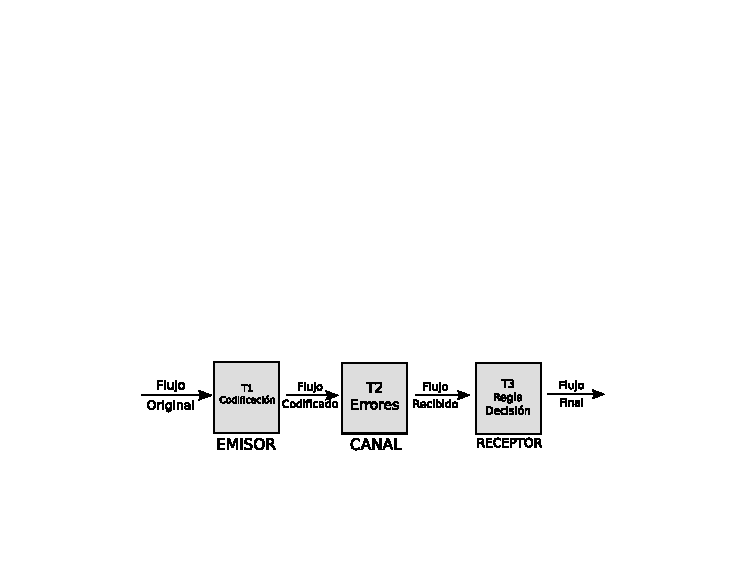
\includegraphics[scale=1]{sistcomunicacion} 
\end{center}
\caption{Un modelo de sistema de comunicación}\label{fig:sistCom2}
\end{figure}

\end{frame} 

%%%%%%%%%%%%%%%%%%%%%%%%%%%%%%%%
\begin{frame}  \small  

\begin{definicion}[Confusión]\label{def:confusion}
Podemos determinar que una confusión ocurre si una palabra codificada en el flujo final no es el mismo que la palabra codificada en la posición correspondiente en el flujo codificado.
\end{definicion}

\begin{itemize} 

\item  Cuando una confusión sucede, el Receptor malinterpreta el mensaje que fue enviado por el Emisor. 

\item Las confusiones son causados por los errores introducidos en la fase T2, transmisión a través de un canal con ruido. 

\item Nuestro propuesta es mostrar que utilizando una elección apropiada del código C en la fase T1, y reglas de decisión adecuadas para C en la fase T3, es \textcolor{red}{posible reducir el número de errores}.

\end{itemize} \end{frame} 

%%%%%%%%%%%%%%%%%%%%%%%%%%%%%%%%
\begin{frame}  \small  
\begin{itemize} 

\item  Por ejemplo, consideramos el escenario descrito anteriormente, donde el Emisor es un controlador emitiendo los símbolos N, S, E, O, utilizando el código $N \mapsto 00$, $S \mapsto 01$, $E \mapsto 10$, $O \mapsto 11$. 

\item El Receptor, divide las palabras de longitud 2, y este caso todas las cuatro posibles palabras de longitud 2 son palabras codificadas $(C=\mathbb{B}^2)$. 

\item Siempre que las palabras codificadas son \textcolor{red}{transmitidas correctamente}, \textbf{no se producen confusiones} cuando el Receptor utiliza \textbf{la regla de decisión}: 

\begin{center}
$\sigma (z)=z$  para todos $z \in \mathbb{B}^2$.
\end{center}

\item Sin embargo, \textcolor{red}{si cualquier bit es transmitido de forma errónea}, entonces las confusiones ocurrirán. 

\item Vamos a ver un ejemplo de una codificación que me permite detectar errores y \textcolor{red}{evitar confusiones}.


\end{itemize} \end{frame} 



%%%%%%%%%%%%%%%%%%%%%%%%%%%%%%%%
\begin{frame}  \small 

\begin{ejemplo}\label{ej:Robot1}

En la situación descrita anteriormente, supongamos que el Emisor utiliza el código

\begin{center}
$N \mapsto 000, S \mapsto 110, E \mapsto 101, O \mapsto 011$,
\end{center}

y el Receptor utiliza la siguiente regla de decisión:

\begin{center}
$\sigma(000) = 000,	\sigma(100) = 011,	\sigma(010) = 000,	\sigma(001) = 101,$
\end{center}
\begin{center}
$\sigma(110) = 110,	\sigma(101) = 101,	\sigma(011) = 011,	\sigma(111) = 110.$
\end{center}

\begin{itemize}
    \item Si una palabra codificada es \textbf{transmitida sin errores}, ¿Es posible encontrar una confusión? 

    \item Si recibimos la palabra 000 y \textbf{asumimos que ocurre un error en un bit}, ¿Es posible que ocurra la confusión?
\end{itemize}

\end{ejemplo}

\end{frame} 



%%%%%%%%%%%%%%%%%%%%%%%%%%%%%%%%
\begin{frame}  \footnotesize
\textit{\underline{Solución}}:\\
\vspace{0.3cm}

\begin{itemize} 

\item  Las reglas de decisión propuestas permiten que cuando tenemos una palabra codificada z obtenemos $\sigma(z)=z$. \textbf{Por tanto si una palabra codificada es transmitida correctamente, no es posible que ocurra ninguna confusión}. 


\item ¿Qué ocurre si un bit en una palabra codificada es transmitida erróneamente? 

\begin{itemize} \footnotesize
\item Note que cada palabra codificada contiene un número de 1's pares (0 ó 2). 

Si tenemos un bit erróneo la palabra tendrá un número impar de 1's y el error puede ser detectado.
\vspace{0.1cm}
\item  Por ejemplo 001 es recibido, entonces el Receptor debe decidir si la palabra codificada era: 
\vspace{0.1cm}\\
000, con un error en el último bit\\ 
101, con un error en el primer bit,\\
011,  con un error en el segundo bit.\\ 
 \vspace{0.1cm}
\item Las reglas de decisión propuestas asumen la segunda posibilidad, y  por tanto si 001 es recibido entonces \textcolor{red}{tenemos una posibilidad que tengamos una confusión}. 
\end{itemize}



\end{itemize} \end{frame} 
%%%%%%%%%%%%%%%%%%%%%%%%%%%%%%%%
\begin{frame}  \footnotesize

\begin{ejemplo}\label{ej:Robot2}

En la misma situación que el anterior supóngase que el Emisor utiliza el código

\begin{center}
$N \mapsto 000000,	S \mapsto 000111,	E \mapsto 111000,	W \mapsto 111111.$
\end{center}

El Receptor utiliza la \textbf{regla de decisión} para cualquier z, $\gamma(z)=c$ es la palabra codificada que se \textcolor{red}{``parece más''} a z, o la palabra codificada c para la cual z y c tienen más bits en común. 

¿En que circunstancia podría ocurrir una confusión?
\end{ejemplo}


\end{frame} 

%%%%%%%%%%%%%%%%%%%%%%%%%%%%%%%%
%%%%%%%%%%%%%%%%%%%%%%%%%%%%%%%%
\begin{frame}  \footnotesize


\textit{\underline{Solución}}:\\
\vspace{0.3cm}
\begin{itemize} 
\item Las palabras codificadas han sido escogidas de forma que si un bit es modificado, la palabra resultante  ``se parece más''  todavía a la palabra codificada original que a cualquier otra palabra codificada.

\item La regla de decisión propuesta hace uso de esta propiedad. 

\item Por ejemplo, si $000000$ es alterado durante la transmisión a $100000$ entonces el Receptor decidirá que recibió $000000$, ya que cualquier otra palabra codificada tendría que haber sido afectada por más de un bit para producir 
$100000$. 

\item Por lo que no solamente detectamos un error en un bit, además es corregido. 

\item \textcolor{red}{Para que ocurra una confusión es necesario que ocurran al menos dos bit erróneos.}
\end{itemize}

\end{frame} 

%%%%%%%%%%%%%%%%%%%%%%%%%%%%%%%%
\begin{frame}  \small 

En resumen, la\textbf{ Comunicación utilizando un canal con ruido},  es un sistema complicado que esta formado por varias etapas.

\begin{enumerate}
\item  \textcolor{red}{Cuantificar los errores} que ocurren cuando los bits en una palabra codificada de longitud n son transmitidas a través de BSC con una probabilidad de error de bit $e$.

\item  Discutir las posibles formas de una \textcolor{red}{regla de decisión}  $\sigma$ que asigna una palabra codificada a cada (posiblemente errónea) palabra recibida.

\item  Tratar de la \textcolor{red}{corrección} de los errores de bit, y como dependen de ciertos parámetros numéricos del código utilizado.
\end{enumerate}

\end{frame} 


%%%%%%%%%%%%%%%%%%%%%%%%%%%%%%%%
%%%%%%%%%%%%%%%%%%%%%%%%%%%%%%%%
%EJERCICIO %%%%%%%%%%%%%%%%%%%%%%%%%%%%%%%
%%%%%%%%%%%%%%%%%%%%%%%%%%%%%%%%

%%%%%%%%%%%%%%%%%%%%%%%%%%%%%%%%
\begin{frame}  \small 

\begin{ejercicio}
En el ejemplo \ref{ej:Robot1} , suponemos que recibimos 111. Si asumimos que solo hay error en un bit, ¿Cuales son las posibilidades para esa instrucción?
\end{ejercicio}


\textit{\underline{Solución}}:\\
\vspace{0.3cm}
Una de las siguientes instrucciones S, E, O.

\end{frame} 

%%%%%%%%%%%%%%%%%%%%%%%%%%%%%%%%
\begin{frame}  \small 

\begin{ejercicio} 
En el ejemplo \ref{ej:Robot2} propusimos una regla de decisión $\gamma$ basada en la idea que $\gamma(z)$ es la palabra codificada que se ``parece más'' a z que cualquier otra palabra codificada. Utilizando esta regla, encuentra los valores de $\gamma(z)$ para la siguientes palabras z:

\begin{center}
101000,	101111,	100111.
\end{center}

\end{ejercicio}


\textit{\underline{Solución}}:\\
\vspace{0.3cm}

$\gamma(101000)$ = 111000; E\\
$\gamma(101111)$ = 111111; O \\
$\gamma(100111)$ = 000111; S\\


\end{frame}  
%%%%%%%%%%%%%%%%%%%%%%%%%%%%%%%%

\begin{frame}  \small 

\begin{ejercicio} 
En el ejemplo \ref{ej:Robot2} suponemos ahora que recibimos la palabra 100100. ¿Es posible realizar una decisión razonable sobre que palabra codificada fue enviada?

\end{ejercicio}


\textit{\underline{Solución}}:\\
\vspace{0.3cm}

En este caso parece que 100100 está más cercana a 000000 que a cualquier otra.

\end{frame}  
%%%%%%%%%%%%%%%%%%%%%%%%%%%%%%%%
%%%%%%%%%%%%%%%%%%%%%%%%%%%%%%%%
%SECCION %%%%%%%%%%%%%%%%%%%%%%%%%%%%%%%
%%%%%%%%%%%%%%%%%%%%%%%%%%%%%%%%


\subsection{El BSC extendido} \label{sec:BSC}

%%%%%%%%%%%%%%%%%%%%%%%%%%%%%%%%
\begin{frame}   \footnotesize
{
\setbeamercolor{block title}{bg=blue!40!black, fg=white}
\setbeamercolor{block body}{bg=white!05, fg=black}
\begin{block}{Sección 5.2.1}
El BSC extendido
\end{block}
}
\end{frame} 
%%%%%%%%%%%%%%%%%%%%%%%%%%%%%%%%
\begin{frame}  \frametitle{El BSC extendido}\small  

\begin{definicion} [Producto del canal]

\begin{itemize}
\item Sea $\Gamma$ y $\Gamma'$ canales con alfabetos de entrada, $I$,$I'$, y alfabetos de salida $J$,$J'$, respectivamente. 

\item El producto del canal $\Gamma'' = \Gamma \times \Gamma'$ tiene alfabeto de entrada $I \times I'$ y alfabeto de salida $J \times J'$, y su matriz es dada por la regla:

\begin{center}
$\Gamma''_{ii'jj'} = \Gamma_{ij} \Gamma'_{i'j'}$
\end{center}

\item En otras palabras $\Gamma''$ es un canal con entradas $ii'$ y salidas $jj'$, y 

\begin{center}
Pr(salida es jj' $|$ entrada es ii') = Pr(j $|$ i) $\times$ Pr(j' $|$ i'). 
\end{center}

\item  En el caso $\Gamma = \Gamma'$, denotamos $\Gamma \times \Gamma'$ como $\Gamma^{2}$ 

\end{itemize}

\end{definicion}

\end{frame} 


%%%%%%%%%%%%%%%%%%%%%%%%%%%%%%%%
\begin{frame}  \footnotesize

\begin{ejemplo}
Supongase que $\Gamma$ es el BSC con probabilidad de error de bit $e$. ¿Cual es la matriz del canal para $\Gamma^2$?
\end{ejemplo}

\textit{\underline{Solución}}:\\

\begin{itemize} 

\item
Las entradas y las salidas para $\Gamma^2$ son los cuatro pares 00, 01, 10, 11. 

\item
Si, por ejemplo, la entrada es 00 y la salida es 10, esto significa que un bit ha sido transmitido de forma errónea ( probabilidad $e$), y un bit ha sido transmitido de forma correcta ($1-e$). 

\item
Por lo que la entrada en la correspondiente posición en $\Gamma^2$ es $e (1-e)$. 

\item 

Utilizando argumentos similares, y etiquetando las filas y columnas en el orden 00, 01, 10, 11, la matriz del canal sería:
\end{itemize} 
\[
\Gamma^2 = \left( \begin{array}{ccccc}
                   
                (1-e)^2  & (1-e) e  & (1-e) e  & e^2 \\
                 (1-e) e  & (1-e)^2 & e^2       &  (1-e) e \\
                 (1-e) e  &  e^2      & (1-e)^2 & (1-e) e \\
                 e^2       & (1-e) e  & (1-e) e  & (1-e)^2  
           \end{array}
    \right) 
\]

\end{frame} 




%%%%%%%%%%%%%%%%%%%%%%%%%%%%%%%%
\begin{frame}  \small  

\begin{definicion}[Canal Extendido]
\begin{itemize} 

\item 
Supongase que dado un canal $\Gamma$ con un conjunto de entrada $I$ y conjunto de salida $J$ y un entero positivo $n$.

\item
Entonces definimos el \textcolor{red}{canal extendido $\Gamma^n$} como el n producto de las copias de $\Gamma$.  

Las entradas a  $\Gamma^n$ son palabras de longitud n en $I$, y las salidas son palabras de longitud $n$ en $J$. 

Si $\Gamma$ es un canal simétrico binario, entonces decimos que $\Gamma^n$ es un \textcolor{red}{BSC extendido}.

\item
Las entradas y salidas para un BSC extendido son los miembros de un conjunto $\mathbb{B}^n$ para todas las palabras binarias de longitud $n$. 

%La siguiente definición es crucial.
\end{itemize}

Podemos obtener una simple fórmula para las entradas de la matriz del canal $\Gamma^n$, generalizando el argumento utilizado anteriormente en el caso n=2. 

\end{definicion}
 \end{frame} 

%%%%%%%%%%%%%%%%%%%%%%%%%%%%%%%%
\begin{frame}  \footnotesize

\begin{definicion}[Distancia Hamming]
Supongase que dados dos palabras $x,y \in \mathbb{B}^n$,

\begin{center}
$x = x_1x_2 \ldots x_n$	$\;\,\,\;\,\,y = y_1y_2 \ldots y_n$.
\end{center}

La \textbf{distancia Hamming d(x, y)} es el número de elementos donde $x$ e $y$ difieren, o es el número de $i$ $(1\leq i \leq n)$ tal que $x_i \neq y_i$.

\end{definicion}

Por ejemplo, considera las siguientes palabras en $\mathbb{B}^7$:

\begin{center}
x = 1010100,	y = 0110100,	z = 1011110.
\end{center}

Las palabras $x$ e $y$ difieren solamente en el primer y segundo bit, por lo que $d(x,y) = 2$. De forma similar $d(x, z) = 3$ y $d(y, z) = 4$.

\begin{teorema}

Sea x,y $\in \mathbb{B}^n$. La entrada $(\Gamma^n)_{xy}$ en el matriz canal para el BSC extendido con la probabilidad de error por bit $e$ es dada por:

\begin{center}
$(\Gamma^n)_{xy} =e^d(1-e)^{n-d}$, donde $d=d(x,y)$.
\end{center}

\end{teorema}

\end{frame} 

%%%%%%%%%%%%%%%%%%%%%%%%%%%%%%%%
%%%%%%%%%%%%%%%%%%%%%%%%%%%%%%%%
%EJERCICIO %%%%%%%%%%%%%%%%%%%%%%%%%%%%%%%
%%%%%%%%%%%%%%%%%%%%%%%%%%%%%%%%

%%%%%%%%%%%%%%%%%%%%%%%%%%%%%%%%
\begin{frame}  \small 
\begin{ejercicio} 
Sea $(\Gamma^2)$ la matriz del canal para el BSC extendido con e=0.01. Calcula los números en las filas de $(\Gamma^2)$ correspondiente a la entrada 00.
\end{ejercicio}

\textit{\underline{Solución}}:\\
\vspace{0.3cm}

Partiendo de $e^d (1-e)^{n-d} $ y que n=2 tenemos $e^d (1-e)^{2-d}$:\\

\begin{itemize}
    \item Si la salida es \textbf{00}: d(00,00) = 0. 
    Por tanto, $e^0 (1-e)^{2}= (1-e)^{2}=(1-0.01)^{2}=0.99^{2}=0.9801$

    \item Si la salida es \textbf{01}: d(00,01) = 1.
    Por tanto, $e^1 (1-e)^{1}= 0.01 (1-0.01)= 0,0099 $

    \item Si la salida es \textbf{10}: d(00,10) = 1.
    Por tanto, $e^1 (1-e)^{1}= 0.01 (1-0.01)= 0,0099 $

    \item Si la salida es \textbf{11}: d(00,11) = 2.
     Por tanto, $e^2 (1-e)^{0}= e^{2}=0.01^{2}=0,0001$
    
\end{itemize}


\end{frame} 


 %%%%%%%%%%%%%%%%%%%%%%%%%%%%%%%%
\begin{frame}  \small 
\begin{ejercicio} 
Describa la matriz de canal para $(\Gamma^2)$  cuando $(\Gamma)$ es el canal binario asimétrico con parámetros a y b.

\end{ejercicio}

\textit{\underline{Solución}}:\\
\vspace{0.3cm}

\[
\Gamma^2 = \left( \begin{array}{ccccc}
                   
                (1-a)^2  & (1-a) a          & (1-a) a  & a^2 \\
                 (1-a) b  & (1-a)(1-b)    & ab       &  a(1-b) \\
                 (1-a) b  &  a b  & (1-a) (1-b) & (1-b) a \\
                 b^2       & b (1-a)  & (1-b) a  & (1-a) (1-b)  
           \end{array}
    \right) 
\]
\end{frame} 




%Sea d la distancia de Hamming. Probar que, para todos  x, y, z \in Bn, d(x, x) = 0,	d(x, y) = d(y, x),	d(x, z) ≤ d(x, y) + d(y, z).[The last property is known as the triangle inequality.]

%%%%%%%%%%%%%%%%%%%%%%%%%%%%%%%%
%%%%%%%%%%%%%%%%%%%%%%%%%%%%%%%%
%SECCION %%%%%%%%%%%%%%%%%%%%%%%%%%%%%%%
%%%%%%%%%%%%%%%%%%%%%%%%%%%%%%%%

\subsection{Reglas Decisión}

%%%%%%%%%%%%%%%%%%%%%%%%%%%%%%%%
\begin{frame}   \footnotesize
{
\setbeamercolor{block title}{bg=blue!40!black, fg=white}
\setbeamercolor{block body}{bg=white!05, fg=black}
\begin{block}{Sección 5.2.2}
Reglas Decisión
\end{block}
}
\end{frame} 
%%%%%%%%%%%%%%
%%%%%%%%%%%%%%%%%%%%%%%%%%%%%%%%
\begin{frame}  \frametitle{Reglas Decisión}\small  
\begin{itemize} 

\item  Anteriormente hemos presentado la idea de \textbf{regla de decisión} $\sigma$ para un código $C \subseteq \mathbb{B}^n$. 


\item La idea es que cuando una recibimos una palabra $z \in \mathbb{B}^n$, el Receptor debe intentar hacer una elección razonable a cual palabra codificada corresponde $\sigma(z) \in C$. 

\item Como ejemplo podemos considerar el código 

\begin{center}
$C = \{000, 110, 101, 011\},$ 
\end{center}

\item  y las \textbf{reglas de decisión arbitrarias} $\sigma$ son:


\begin{center}
$\sigma$(000) = 000,	$\sigma$(100) = 011,	$\sigma$(010) = 000,	$\sigma$(001) = 101, 
\end{center}
\begin{center}
$\sigma$(110) = 110,	$\sigma$(101) = 101,	$\sigma$(011) = 011,	$\sigma$(111) = 110.
\end{center}

\end{itemize} \end{frame} 

%%%%%%%%%%%%%%%%%%%%%%%%%%%%%%%%
\begin{frame}  \small  
\begin{itemize} 

\item  Ya que la palabra $011$ es una palabra codificada, es razonable definir $\sigma$(011) = 011. 

\item  Por otro lado, $100$ no es una palabra codificada, y estableciendo  $\sigma$(100) = 011 asumimos que un error ha ocurrido en los tres  bits, lo cual es \textcolor{red}{claramente poco probable}.

\item  Una buena regla de decisión depende del sistema de comunicación, en particular, el código C y la matriz del canal $\Gamma$. 


\item El Receptor debe utilizar esta información para formular una regla de decisión que proporcione la mejor opción de establecer la elección adecuada.

\vspace{0.7cm}

\begin{definicion}[Regla del Observador Ideal]
La regla del observador ideal dice que, dado z, el Receptor debería escoger $\sigma(z)$ igual a una palabra codificada $c$ con la máxima probabilidad que $c$ fue enviada teniendo $z$.
\end{definicion}

\end{itemize} \end{frame}

%%%%%%%%%%%%%%%%%%%%%%%%%%%%%%%%
\begin{frame}  \footnotesize
\begin{itemize} 

\item Desafortunadamente, \textcolor{red}{las probabilidades condicionales que implica esta definición son de la forma $Pr (c | z)$ y no tienen por que estar disponibles al Receptor}.

\item  Para calcular $Pr (c | z)$ es necesario igualar las dos expresiones para la probabilidad $t_{cz}$ de un par entrada-salida (c,z):

\begin{center}
$t_{cz}	= q_z Pr(c | z)$	      

$t_{cz}= p_c Pr(z | c)$.
\end{center}

\item  Por definición $Pr(z | c)$ es el término $\Gamma_{cz}$ en la matriz del canal. 

\item Sin embargo  $Pr(c | z)$ =$ p_c\Gamma_{cz}/ q_z$  involucra la distribución de entrada $p$ así como $\Gamma$. 

\item En general \textcolor{red}{las características de la entrada no son conocidas en el Receptor}, pero si las las características del canal, en particular las probabilidades  $\Gamma_{cz}=Pr(z | c)$. 

\item Por tanto podemos definir una regla más práctica de la siguiente forma:
   
\end{itemize} \end{frame} 


%%%%%%%%%%%%%%%%%%%%%%%%%%%%%%%%
\begin{frame}  \footnotesize

\begin{definicion}[Regla de la máxima posibilidad]
La regla de la máxima posibilidad dice que, dado z, el Receptor debería escoger $\sigma(z)$ igual a una palabra codificada $c$ que cumpla 

\begin{center}
$Pr(z|c) \geq Pr(z|c')$ para todo $c' \in C$.
\end{center}
\end{definicion}

%x\begin{itemize} 

\begin{definicion}[Regla de la Mínima distancia]
La regla de la mínima distancia (o regla MD) dice que dado $z \in \mathbb{B}^n$, el Receptor debe escoger  $\sigma(z)$ sea una palabra codificada $c$ tal que $d(z,c)$ es mínimo. 
\end{definicion}

\begin{teorema}
Para un BSC extendido con $e < 1/2$, la regla de la máxima posibilidad es equivalente a la regla MD.
\end{teorema}

%\item  La regla de la máxima posibilidad dice que $\sigma(z)$ debe ser una palabra codificada $c$ para la cual la probabilidad que $z$  sea recibida, dada que $c$ es enviada debe ser máxima.

%\item Escribiendo la condición como $\Gamma_{cz} \geq  \Gamma_{c'z} $ la regla puede ser expresada:

%	\begin{itemize} 
%		\item Dado $z$, escoger el mayor término $\Gamma_{cz}$ en la columna $z$ de la matriz del canal y establece $\sigma(z)=c$. 
%	\end{itemize}

%\item En el caso que exista más de una $c$ que satisfaga esta condición, el receptor deberá escoger una de forma arbitraria. 

%\item Cuando el canal es BSC extendido, tenemos una fórmula para los elementos de una matriz del canal, y esto permite una interpretación simple de la regla de la máxima posibilidad.

%\end{itemize} 
\end{frame} 

%%%%%%%%%%%%%%%%%%%%%%%%%%%%%%%%
%\begin{frame}  \small  

%\begin{definicion}[Regla de la Mínima distancia]
%La regla de la mínima distancia (o regla MD) dice que dado $z \in \mathbb{B}^n$, el %Receptor debe escoger  $\sigma(z)$ sea una palabra codificada $c$ tal que $d(z,c)$ es %mínimo. 
%\end{definicion}

%\begin{teorema}
%Para un BSC extendido con $e < 1/2$, la regla de la máxima posibilidad es equivalente %a la regla MD.
%\end{teorema}


%\end{frame} 
%%%%%%%%%%%%%%%%%%%%%%%%%%%%%%%%
\begin{frame}  \small  
\begin{ejemplo} 
Supongamos que el código $C \subseteq \mathbb{B}^8$ tiene siete palabras codificadas 

\begin{center}
 $c_1$ =0000 0000 $c_2$ =0011 1000 $c_3$ =1100 0001 $c_4$ =0000 1110
\end{center}
\begin{center}
$c_5$ = 1011 1011	$c_6$ = 0011 0110	$c_7$ = 1100 1011. 
\end{center}

Si $\sigma$ es la \textbf{regla MD}, ¿Qué valor debe asignar el Receptor a:

\begin{center}
(i)	$\sigma$(1010 1011)	(ii)	$\sigma$(1100 1001) ?
\end{center}


\end{ejemplo}

\end{frame} 

%%%%%%%%%%%%%%%%%%%%%%%%%%%%%%%%
\begin{frame}  \small  
\vspace{0.3cm}
\textit{\underline{Solución}}:\\

(i) Las distancias $d(z, c_i)$ para z = 1010 1011 son:

\[
 \begin{array}{lccccccc}
               i:  & 1  & 2  & 3 & 4  & 5  & 6 & 7 \\
        d(z,c_i): & 5  & 4  & 4 & 4  & 1  & 5 & 2 
           \end{array}
           \]

Por tanto la palabra codificada a z es $c_5$= 1011 1011. Acorde con el teorema, esta es también la palabra codificada $c$ para la cual la probabilidad de recibir $z$, dado que $c$ fue enviada, es la mayor.

\vspace{0.3cm}

(ii) Las distancias $d(z', c_i)$ para  z' = 1100 1001 son:

\[
 \begin{array}{lccccccc}
               i:  & 1  & 2  & 3 & 4  & 5  & 6 & 7 \\
        d(z,c_i): & 4  & 5  & 1 & 5  & 4  & 8 & 1 
           \end{array}
           \]

En este caso tenemos dos palabras codificadas $c_3$ y $c_7$ que pueden ser escogidas como $\sigma(z')$. El Receptor puede fijar una de las dos opciones, o cuando $z'$ ocurre, elegirá una de las dos opciones de forma aleatoria.


\end{frame} 
%%%%%%%%%%%%%%%%%%%%%%%%%%%%%%%%
%%%%%%%%%%%%%%%%%%%%%%%%%%%%%%%%
%EJERCICIO %%%%%%%%%%%%%%%%%%%%%%%%%%%%%%%
%%%%%%%%%%%%%%%%%%%%%%%%%%%%%%%%

%%%%%%%%%%%%%%%%%%%%%%%%%%%%%%%%
\begin{frame}  \small 
\begin{ejercicio} 

Sea $C \subseteq \mathbb{B}^8$ con palabras codificadas como:

\begin{center}
 $c_1 =0000 0000$ $c_2 =0011 1000$ $c_3 =1100 0001$ $c_4 =0000 1110$
\end{center}
\begin{center}
$c_5 = 1011 1011$	$c_6 = 0011 0110$	$c_7 = 1100 1011$. 
\end{center}

Utilizando la regla MD $\sigma$, encontrar $\sigma(z)$ cuando z es i) 1000 1011,	ii) 1011 1010,	iii) 1100 0101.

\end{ejercicio}

\end{frame} 
%%%%%%%%%%%%%%%%%%%%%%%%%%%%%%%%
\begin{frame}  \small 

\textit{\underline{Solución}}:\\
\vspace{0.3cm}

i) $1000 1011 \mapsto c_7$
\[
 \begin{array}{lccccccc}
               i:  & 1  & 2  & 3 & 4  & 5  & 6 & 7 \\
        d(z,c_i): & 4  & 5  & 3 & 3  & 2  & 6 & 1 
           \end{array}
           \]

ii) $1011 1010 \mapsto c_5$
\[
 \begin{array}{lccccccc}
               i:  & 1  & 2  & 3 & 4  & 5  & 6 & 7 \\
        d(z,c_i): & 5  & 2 & 6 & 4  & 1  & 3 & 4 
           \end{array}
           \]

iii) $1100 0101 \mapsto c_3$
\[
 \begin{array}{lccccccc}
               i:  & 1  & 2  & 3 & 4  & 5  & 6 & 7 \\
        d(z,c_i): & 4  & 7  & 1 & 5  & 6  & 6 & 2 
           \end{array}
           \]
\end{frame} 

%%%%%%%%%%%%%%%%%%%%%%%%%%%%%%%%
\begin{frame}  \small 
\begin{ejercicio} 

Considere el código C 	que consiste de 10 palabras en $\mathbb{B}^5$ que tienen exactamente  dos bits igual a 1. Si un error es realizado en la transmisión del código, 
\vspace{0.1cm}
¿Cuales son las posibles palabras recibidas?. 
\vspace{0.1cm}
Para cada z, realizar una lista de palabras codificadas que están cercas a z.

\end{ejercicio}

\end{frame} 


%%%%%%%%%%%%%%%%%%%%%%%%%%%%%%%%
\begin{frame}  \small 

\textit{\underline{Solución}}:\\

Las palabras del código son: 

\begin{center}
$c_1=11000$, $c_2=10100$, $c_3=10010$, $c_4=10001$, $c_5=01100$, $c_6=01010$, $c_7=01001$, $c_8=00110$, $c_9=00101$, $c_{10}=00011$.
\end{center}

Si transmito 11000 y hay un error los posibles palabras codificadas erróneas son:

\begin{center}
 $z_1=$10000, $z_2=$01000, $z_3=$11100, $z_4=$11010, $z_5=$11001
\end{center}

En el caso de $z_1=10000$
\[
 \begin{array}{lcccccccccc}
                 i:  & 1  & 2  & 3 & 4  & 5  & 6 & 7  & 8 & 9 & 10 \\
        d(z,c_i): & 1  & 1  & 1 & 1  & 3  & 3 & 3  & 3  & 3   &3 
           \end{array}
           \]
\end{frame} 


%6.9. Under the same conditions as in the previous exercise, suppose the Receiver uses the MD rule, with the proviso that if there are k code- words that are nearest to a given word z, one of them is chosen as σ(z) with probability 1/k. Suppose the codeword 11000 is sent, and probability of a single bit-error in transmission is e. Show that there is probability 7e/12 that the Receiver will decide (wrongly) that the codeword sent was 10001.

%6.10. Let Γ be a binary asymmetric channel with property that 0 is al- ways transmitted correctly, but 1 is transmitted as 0 with probability f (0 < f < 1). Write down the entries (Γ3)cz of the extended chan- nel matrix that correspond to codewords in the code C = {000, 111}. What is the maximum likelihood decision rule for C, using this chan- nel?

%6.11. Show that the maximum likelihood rule is not the same as the MD rule for the channnel considered in the previous exercise.

%%%%%%%%%%%%%%%%%%%%%%%%%%%%%%%%
%%%%%%%%%%%%%%%%%%%%%%%%%%%%%%%%
%SECCION %%%%%%%%%%%%%%%%%%%%%%%%%%%%%%%
%%%%%%%%%%%%%%%%%%%%%%%%%%%%%%%%


\subsection{Corrección Errores}
%%%%%%%%%%%%%%%%%%%%%%%%%%%%%%%%
\begin{frame}   \footnotesize
{
\setbeamercolor{block title}{bg=blue!40!black, fg=white}
\setbeamercolor{block body}{bg=white!05, fg=black}
\begin{block}{Sección 5.2.3}
Corrección Errores
\end{block}
}
\end{frame} 

%%%%%%%%%%%%%%%%%%%%%%%%%%%%%%%%
\begin{frame}  \frametitle{Corrección Errores}\small 



 
\begin{itemize} 

\item  El propósito de una regla de decisión es asegurar que, tanto como sea posible, los errores sean corregidos. 

\item Nos centraremos en la regla MD para BSC extendido, donde la efectividad de la regla depende de ciertos parámetros del código.

\end{itemize} 

\begin{definicion}[Mínima Distancia] 
Sea d(c,c') la distancia Hamming entre dos palabras codificadas c y $c'$ en un código $C \subseteq \mathbb{B}^n$. 

La \textbf{mínima distancia} de C es 

\begin{center}
$\delta= min$ $d(c, c')$ para todo $c \neq c'$
\end{center}

\end{definicion}

\end{frame} 

%%%%%%%%%%%%%%%%%%%%%%%%%%%%%%%%
\begin{frame}  \small  


\begin{itemize} 

\item  Por ejemplo, supóngase $C \subseteq \mathbb{B}^6$ tiene cuatro palabras codificadas 
\begin{center}
 000 000, 111 000, 001 110, 110 011
\end{center}

\item La distancia entre las palabras codificadas son como sigue:

\begin{center}
$d(000 000, 111 000) = 3$,	$d(000 000, 001 110) = 3$,	$d(000 000, 110 011) = 4$,
$d(111 000, 001 110) = 4$,	$d(111 000, 110 011) = 3$,	$d(001 110, 110 011) = 5$.
\end{center}

\item  por lo que la mínima distancia es  $\delta = 3$.
\end{itemize} 

	


\end{frame} 

%%%%%%%%%%%%%%%%%%%%%%%%%%%%%%%%
\begin{frame}  \small  

\begin{definicion} [Vecindario]
Para cualquier $x \in \mathbb{B}^n$ y cualquier $r \geq 0$, el vecindario de x con radio r es el conjunto 
\begin{center}
$N_r(x)=\{y \in \mathbb{B}^n$ $|$ $d(x,y)\leq r \}.$
\end{center}
\end{definicion}

\begin{itemize} 

\item  \textcolor{red}{El vecindario $N_r(x)$ contiene todas las palabras que pueden ser obtenidos desde $x$ no cometiendo más de r bit errores.} 

\item Por ejemplo, si establecemos $x=11010 \in \mathbb{B}^5$. 
\begin{itemize} 
\item El vecindario $N_1(x)$ contiene x y las cinco palabras obtenidas al realizar un error en $x$, 
\item $N_1(x)$ = \{11010, 01010, 10010, 11110, 11000, 11011\}.
\end{itemize} 

\end{itemize} 
\end{frame} 

%%%%%%%%%%%%%%%%%%%%%%%%%%%%%%%%
\begin{frame}  \small 

\begin{lema}
Si C es un código con $\delta \geq 2r+1$, entonces para cada palabra codificada $c, c' \in C$, el vecindario $N_r(c)$ y $N_r(c')$ son disjuntos (Vea figura \ref{fig:vecindario}).
\end{lema}

\begin{figure}[!hbtp]
\begin{center}
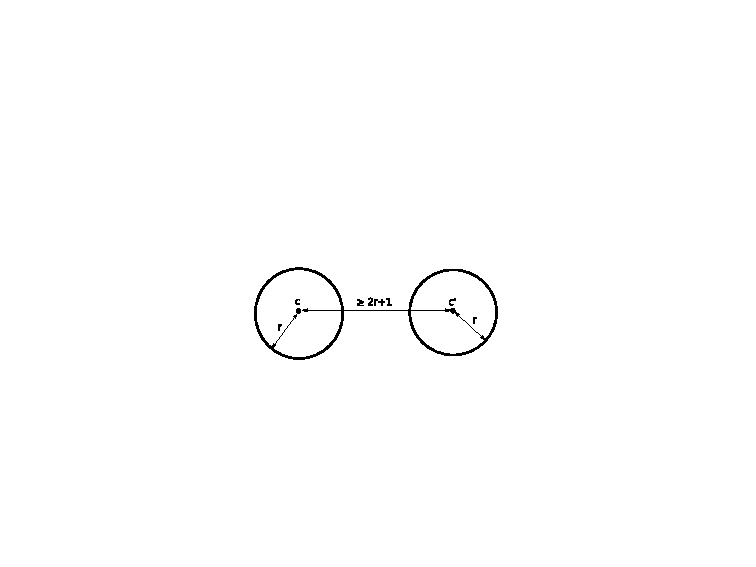
\includegraphics[scale=1]{vecindario} 
\end{center}
\caption{Si $\delta \geq 2r+1$ entonces $N_r(c)$ y $N_r(c')$ son disjuntos}\label{fig:vecindario}
\end{figure}

\end{frame} 

%%%%%%%%%%%%%%%%%%%%%%%%%%%%%%%%
\begin{frame}  \small  

\begin{teorema}
Si el Emisor utiliza un código C que tiene la \textbf{mínima distancia} $\delta \geq 2r+1$, y el Receptor utiliza la \textbf{regla MD}. 
\vspace{0.3cm}

\textbf{No existe confusión} si no se produzcan error en más de \textbf{r bits} en la transmisión de cualquier palabra codificada.
\vspace{0.3cm}

\textbf{Cada palabra recibida será restaurada a una palabra codificada correcta}. 
\end{teorema}

\begin{definicion} [Código Corrector Error]
Un código $C \subseteq \mathbb{B}^n$ es un código corrector de error r si $\delta \geq 2r+1$.
\end{definicion}	

\begin{itemize}
\item La definición esta basada en la suposición que utilizamos la \textbf{regla MD}. 
\item Un código con $\delta \geq 2r+1$ corrige r errores, por ejemplo, si $\delta$ es  3, entonces C corrige 1 error.
\end{itemize}




\end{frame} 
%%%%%%%%%%%%%%%%%%%%%%%%%%%%%%%%
%%%%%%%%%%%%%%%%%%%%%%%%%%%%%%%%
%EJERCICIO %%%%%%%%%%%%%%%%%%%%%%%%%%%%%%%
%%%%%%%%%%%%%%%%%%%%%%%%%%%%%%%%

%%%%%%%%%%%%%%%%%%%%%%%%%%%%%%%%
\begin{frame}  \footnotesize \begin{ejercicio} 
Construya un código corrector-1 $C \subseteq \mathbb{B}^6$ con $|C| =5$.
\end{ejercicio}


\textit{\underline{Solución}}:\\

\vspace{0.3cm}
En el ejemplo anterior teníamos 

\begin{center}
 000 000, 111 000, 001 110, 110 011
\end{center}

 La distancia eran:

\begin{center}
$d(000 000, 111 000) = 3$,	$d(000 000, 001 110) = 3$,	$d(000 000, 110 011) = 4$,
$d(111 000, 001 110) = 4$,	$d(111 000, 110 011) = 3$,	$d(001 110, 110 011) = 5$.
\end{center}

Debemos añadir una palabra, longitud 5. Es posible añadir 010 101.

\begin{center}
$d(000 000, 010 101) = 3$,	$d(111 000, 010 101) = 4$,	

$d(001 110, 010 101) = 4$, $d(110 011, 010 101) =3$.
\end{center}

por lo que la mínima distancia sigue siendo  $\delta = 3$.

\end{frame} 

%%%%%%%%%%%%%%%%%%%%%%%%%%%%%%%%
\begin{frame}  \small 

\begin{ejercicio} 

Para el código C construido en el ejercicio anterior, ¿Cuantas palabras no pueden ser corregidas bajo el supuesto que hemos realizado la corrección de al menos un bit?

\end{ejercicio} 


\textit{\underline{Solución}}:\\
\vspace{0.3cm}
Para cada $c \in C$, hay 6 palabras que pueden ser derivadas con un sólo error, por lo que $|N_1(c)|=7$.

\vspace{0.3cm}

Por tanto, con las 5 palabras tenemos 5 x 7 = \textbf{35 palabras que pueden ser corregidas}, por lo que el número de palabras que \textbf{no pueden ser corregidas son $2^6 - 35 = 29$}.

 \end{frame} 

%6.14. Is the code with |C| = 5 constructed in Exercise 6.12 the largest possible 1-error-correcting binary code with words of length 6?

%%%%%%%%%%%%%%%%%%%%%%%%%%%%%%%%
%\begin{frame}  \small \begin{ejercicio} \end{ejercicio} \textit{\underline{Solución}}:\\ \end{frame} 

%%%%%%%%%%%%%%%%%%%%%%%%%%%%%%%%
%%%%%%%%%%%%%%%%%%%%%%%%%%%%%%%%
%SECCION %%%%%%%%%%%%%%%%%%%%%%%%%%%%%%%
%%%%%%%%%%%%%%%%%%%%%%%%%%%%%%%%


\subsection{El límite de embalaje (The packing bound)}

\begin{frame}   \footnotesize
{
\setbeamercolor{block title}{bg=blue!40!black, fg=white}
\setbeamercolor{block body}{bg=white!05, fg=black}
\begin{block}{Sección 5.2.4}
El límite de embalaje (The packing bound)
\end{block}
}
\end{frame} 
%%%%%%%%%%%%%%%%%%%%%%%%%%%%%%%%
\begin{frame}  \frametitle{El límite de embalaje (The packing bound)}\footnotesize  
\begin{itemize} 




\item  Construir códigos correctores con un $\delta$ dado, implica una restricción en  el número de palabras codificadas $|C|$, ya que las palabras codificadas deben estar suficientemente separadas. 

\begin{teorema}[Límite de embalaje]

Si $C \subseteq \mathbb{B}^n$ es un código con $\delta \geq 2r+1$, entonces:

\begin{center}
    $ |C| \times V(n,r)    	\leq 2^n  $		
\end{center}

donde $V(n,r) = \sum_{i=0}^{r} \binom{n}{i} = 1 + n + \binom{n}{2} + \cdots + \binom{n}{r}$

\vspace{0.4cm}

\tiny
 $\binom{n}{r}$  es el coeficiente binomial, y representa el número de formas de elegir r elementos de un conjunto de n y es calculado como $=\frac{n!}{r! (n-r)!}$

\end{teorema}
%(n x) n! / x! (n-x)!


\item  $A(n,\delta)$ es el mayor valor de $|C|$ para el cual existe un código $C \subseteq \mathbb{B}^n$ con mínima distancia $\delta$.  
\[
A(n, \delta) = \max \left\{\, |C| : C \subseteq \mathbb{B}^n,\; d_{\min}(C) \ge \delta \,\right\}
\]
\item El límite de embalaje nos proporciona un límite superior para $A(n,\delta)$, pero no tenemos garantía que un código de ese tamaño exista. 

\item Determinar qué subconjunto máximo cumple que todas las distancias $ \geq delta$  es un problema \textbf{NP-hard}.

\end{itemize} 

\end{frame} 

%%%%%%%%%%%%%%%%%%%%%%%%%%%%%%%%
\begin{frame}  \small  
\begin{ejemplo}
Debemos emitir número de ID, de la forma de cadenas de n bits, a 100 empleados. Los empleados pueden cometer errores utilizando sus ID's, por lo que hemos decidido que debemos utilizar un código corrector de 2 bits. ¿Cual es el menor valor de n para que esto sea posible?
\end{ejemplo}


\textit{\underline{Solución}}:\\
\vspace{0.3cm}
Para r = 2 errores y $|C| = 100$ el límite de embalaje 

\[
  100 \left( 1+n+  n (n-1) /2 \right)   \leq 2^n   =  50(n^2 +n+2) \leq 2^n 		
\]
\vspace{0.3cm}

Por prueba y error, el menor valor de n que mantiene esta inegualdad es n=14. 
\vspace{0.3cm}

Por supuesto, el problema de construir un  conjunto con 100 palabras codificadas, cada una de longitud 14, se mantiene.


\end{frame} 



%%%%%%%%%%%%%%%%%%%%%%%%%%%%%%%%
\begin{frame}  \small  

\begin{ejemplo}
¿Cual es el valor de $A(10, 7)$, el tamaño más grande posible de un código $C \subseteq \mathbb{B}^{10}$ con una distancia mínima $\delta = 7$?
\end{ejemplo}



\textit{\underline{Solución}}:\\
\vspace{0.3cm}
En este caso necesitamos $\delta = 2r+1$ con r=3, por lo que el límite de embalaje es

\[
 |C| \left( 1+10+ 
            \left( \begin{array}{c}
                  10 \\
                  2       
           			\end{array}
    		\right) + 
    		\left( \begin{array}{c}
                  10  \\
                  3      
           			\end{array}
    		\right)    		
    \right)    	\leq 2^{10}    		
\]

que es, $|C| \leq 1024/176$. Ya que $|C|$  es un entero, tendremos que $A(10, 7) \leq 5$

%In fact A(10, 7) = 2. To prove this, we can suppose without loss of generality that one codeword is 0000000000. Then any other codeword must have at least 7 ones. Now two words of length 10 with at least 7 ones must have at least 4 ones in the same positions. Hence if these words are distinct, their distance can be at most 6, contrary to the condition δ = 7. It follows that there can be only one other codeword besides 0000000000.

\end{frame} 

%%%%%%%%%%%%%%%%%%%%%%%%%%%%%%%%
\begin{frame}  \small  


\begin{itemize} 

\item  Otro punto de vista del límite de embalaje, es la \textbf{Tasa de Información}.

\item  $C\subseteq \mathbb{B}^n$ y $|C| = m$, una palabra codificada $c \in C$ transmite  \textcolor{red}{$log_2 \times m$ bits de información}, pero requiere \textbf{n bits de datos}.


\end{itemize}

\begin{definicion}[Tasa de Información]

La tasa de información de un código $C \subseteq \mathbb{B}^n$ es

\begin{center}
$\rho = \frac{log_2|C|}{n}$
\end{center}
\end{definicion}


Supongamos $C \subseteq \mathbb{B}^6$ tiene cuatro palabras codificadas

\begin{center}
000000, 111000, 001110, 110011.
\end{center}

 En este caso n=6 y $|C| = 4 = 2^2$, la tasa de información  es $\rho = 2/6 = 1/3$.  \\
\vspace{0.2cm}

  C requiere 6 bits de datos para codificar 2 bits de información. \\

\vspace{0.2cm}

 Construir un código  $C \subseteq \mathbb{B}^n$  con un  tamaño dado $|C|$ y dado un valor dado de $\delta$ es equivalente a construir un código con valores dados de n, $\rho$ y $\delta$. 

 \end{frame} 

%%%%%%%%%%%%%%%%%%%%%%%%%%%%%%%%

\begin{frame}[fragile]  {vnr\_packing\_plot.py}\footnotesize  

\begin{figure}[!tb]
  \begin{center}
    \subfigure[python3 vnr\_packing\_plot.py 10 -r 2]{
    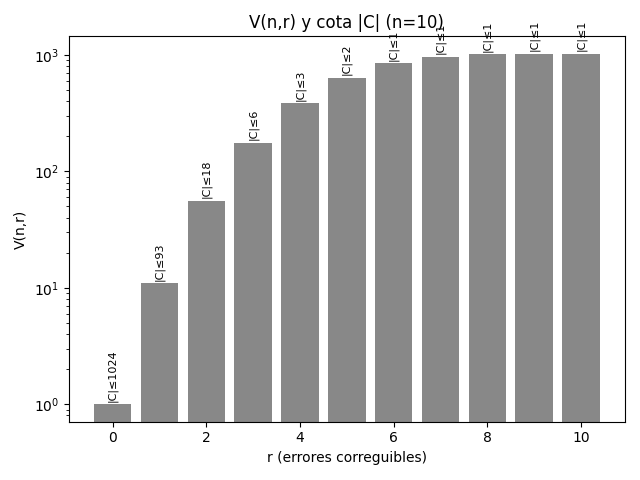
\includegraphics[width=0.45\linewidth]{V(10,r).png}}
    \subfigure[python3 vnr\_packing\_plot.py 100 20]{
    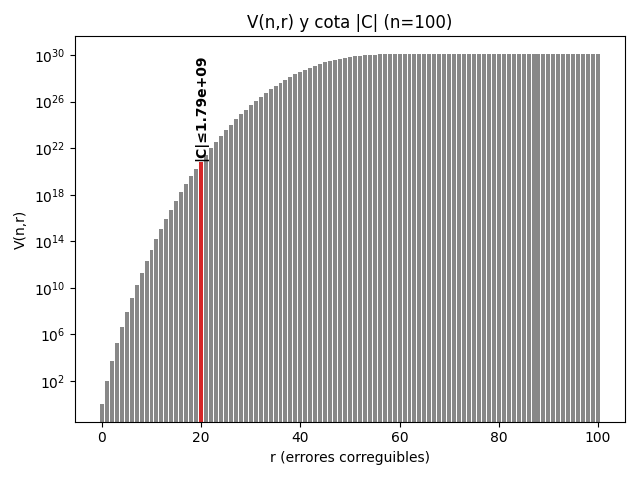
\includegraphics[width=0.45\linewidth]{V(100,20).png}}
  \end{center}
\end{figure}

\begin{enumerate}\footnotesize
  \item \textbf{Reutilizar el script \texttt{vnr\_packing\_plot.py}:}
  \begin{itemize}
    \item Cambiar el valor de $n$ y observar cómo crece $V(n,r)$.
    \item Resaltar distintos valores de $r$ en la gráfica.
  \end{itemize}
   \item \textbf{Calcular y graficar para varios valores de $n$:}
    V(n,r), $|C|$, $\rho$.
   \item \textbf{Generar una tabla o gráfico comparativo} que muestre la evolución de la tasa de información $\rho$ para distintos valores de $r$. Añadir un eje secundario en la gráfica con la tasa de información $\rho$.
\end{enumerate}

\end{frame} 
%%%%%%%%%%%%%%%%%%%%%%%%%%%%%%%%
%%%%%%%%%%%%%%%%%%%%%%%%%%%%%%%%
%EJERCICIO %%%%%%%%%%%%%%%%%%%%%%%%%%%%%%%
%%%%%%%%%%%%%%%%%%%%%%%%%%%%%%%%

%%%%%%%%%%%%%%%%%%%%%%%%%%%%%%%%
\begin{frame}  \small \begin{ejercicio} 

Si necesitamos un código  $C \subseteq \mathbb{B}^6$ con tasa de información de al menos 0.35, ¿Cual es el menor valor posible de $|C|$?

\end{ejercicio} 

\textit{\underline{Solución}}:\\ 
\vspace{0.3cm}

$\rho=\frac{log_2|C|}{n}$; \\
\vspace{0.2cm}
$0.35=\frac{log_2|C|}{6}$ \\
\vspace{0.2cm}
$2,1 =log_2 |C|$ \\
\vspace{0.2cm}
$|C| \geq 2^{2.1} $ \hspace{0.2cm} $2^{2.1} = 2^2 \times 2^{0.1} = 4 \times 1.07 = 4.287$

\vspace{0.2cm}

Por tanto $|C|=5$\\

\end{frame} 

%%%%%%%%%%%%%%%%%%%%%%%%%%%%%%%%
\begin{frame}  \small \begin{ejercicio} 
Muestra que $(log_2 \; 9)/6 = 0.528$ es un límite superior para la tasa de información de un código $C\subseteq \mathbb{B}^6$ corrector 1

\end{ejercicio} \textit{\underline{Solución}}:\\ 
\vspace{0.3cm}
Según el límite del embalaje tenemos 
$|C| (1+n) \leq 2^6 = \;\; 7 |C| \leq 64 ;$ 

Por tanto $|C| \leq 9$ y la tasa es $\rho = log_2 \; 9 /6$

\end{frame} 



%%%%%%%%%%%%%%%%%%%%%%%%%%%%%%%%
\begin{frame}  \small \begin{ejercicio} 

Queremos emitir números ID, en la forma de cadena de n bits, a 1000 personas, utilizando un código corrector-1.¿Cual es el menor valor para n que hace esta situación posible? 

\end{ejercicio} 



\textit{\underline{Solución}}:\\ 

\vspace{0.3cm}

Tenemos $|C|=1000$ personas  y r=1.\\
\vspace{0.3cm}
Por lo que el límite de embalaje nos proporciona
$1000 (1+n) \leq 2^n; 1000+1000n \leq 2^n$; \\
\vspace{0.3cm}
Con n=14 tenemos $15000 \leq 16384$


\end{frame} 







%%%%%%%%%%%%%%%%%%%%%%%%%%%%%%%%
%\begin{frame}  \small \begin{ejercicio} \end{ejercicio} \textit{\underline{Solución}}:\\ \end{frame} 


%6.18. Using a general form of the proof that A(10, 7) = 2 (Example 6.22), show that if δ > 2n/3 then A(n,δ) = 2.


%6.19. Prove that there is an r-error-correcting code C ⊆ Bn satisfying |C|��1+n+��n��+···+��n���� ≥ 2n. 2 2r [This result gives a lower bound for A(n, 2r + 1). It is known as the Gilbert-Varshamov bound.]

%6.20. An r-error-correcting code C ⊆ Bn is said to be perfect if the neigh- bourhoods Nr(c) exactly cover Bn – that is, every word in Bn is in precisely one Nr(c). Show that if r = 1 and such a code exists, then n must be of the form 2m − 1. [See also Section 9.1.]


%%%%%%%%%%%%%%%%%%%%%%%%%%%%%%%%
%%%%%%%%%%%%%%%%%%%%%%%%%%%%%%%%
%SECCION %%%%%%%%%%%%%%%%%%%%%%%%%%%%%%%
%%%%%%%%%%%%%%%%%%%%%%%%%%%%%%%%


\section{La probabilidad de una confusión}


\begin{frame}   \footnotesize
{
\setbeamercolor{block title}{bg=blue!60!black, fg=white}
\setbeamercolor{block body}{bg=blue!10, fg=black}
\begin{block}{Sección 3}
La probabilidad de una confusión
\end{block}
}
\end{frame} 

%%%%%%%%%%%%%%%%%%%%%%%%%%%%%%%%
\begin{frame}  \frametitle{La probabilidad de una confusión}\small  

Volvemos (Figura \ref{fig:sistCom}) al modelo de comunicaciones anteriormente descrito. 


\begin{figure}[!hbtp]
\begin{center}
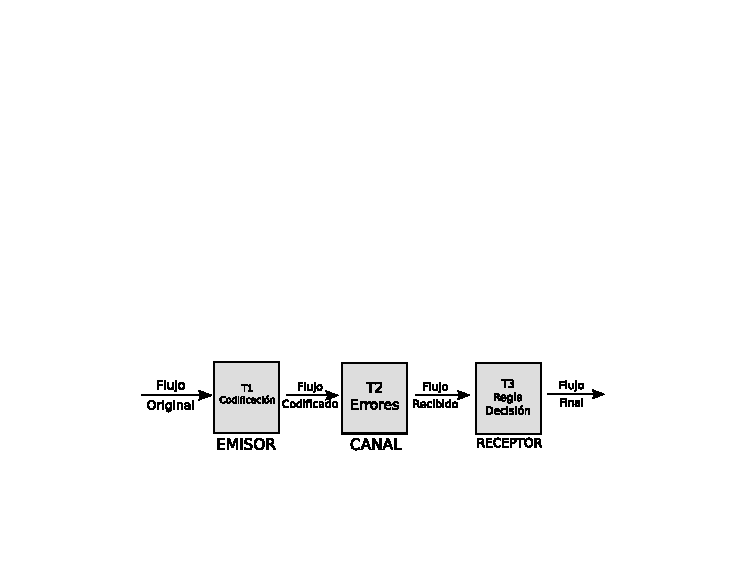
\includegraphics[scale=1]{sistcomunicacion} 
\end{center}
\caption{Un modelo de sistema de comunicación}\label{fig:sistCom}
\end{figure}

\begin{itemize} \footnotesize

\item Flujo original es emitido por una fuente que produce símbolos de un alfabeto X, siguiendo distribución de probabilidad $p$ .

\item Emisor utiliza el código $C$, la probabilidad de enviar $c \in C$ =  probabilidad fuente emita el símbolo $x \in X$ para el cual c es la palabra codificada.  Por tanto,  Flujo codificado como emitido por una fuente (C,p). 

\item El canal es el BSC extendido y el Receptor utiliza la regla MD.

\item Para cada $c \in C$, denotamos por F(c) el conjunto de palabras las cuales la regla MD $\sigma$ no asigna c:
\end{itemize}

\begin{center}
$F(c)=\{z \in \mathbb{B}^n | \sigma (z) \neq c\}$.
\end{center}


\end{frame} 


%%%%%%%%%%%%%%%%%%%%%%%%%%%%%%%%
\begin{frame}  \footnotesize
\begin{itemize} 

\item   Una \textcolor{red}{confusión} (Def. \ref{def:confusion}) ocurre cuando una palabra codificada $c \in C$ es alterada en transmisión y la palabra recibida está en F(c). 

\item  Receptor decidirá una palabra codificada $c'$ diferente de la c que fue enviada. 

\item  $M_c$ la probabilidad cuando palabra codificada \textit{c} es enviada y la palabra recibida z está en F(c), $M_c$ es la suma de las probabilidades condicionales $Pr(z | c)$ para  $z \in F (c)$:


\begin{center}
$M_c = \sum_{z \in F(c) } Pr(z | c)$ 
\end{center}
\end{itemize}
\begin{definicion}[Probabilidad de una confusión]

La probabilidad de una confusión cuando el flujo codificado corresponde a una fuente $(C,p)$

\begin{center}
$M (C,p) =  \sum_{c \in C } p_c M_c$ 
\end{center}

\end{definicion}
\vspace{0.3cm}

\textcolor{red}{El objetivo es escoger el código C para que M(C,p) sea tan pequeño como sea posible.} 
 \end{frame} 

%%%%%%%%%%%%%%%%%%%%%%%%%%%%%%%%
\begin{frame}  \small  

\begin{ejemplo}
Estamos realizando un mando para manejar una aplicación remota y debemos mandar solamente dos mensajes $ARRIBA$, $ABAJO$. Tenemos dos posibles códigos:

\begin{center}
(i) $ARRIBA \mapsto 0$,  $ABAJO \mapsto 1$;   

(ii) $ARRIBA \mapsto 000$,  $ABAJO \mapsto 111$; 
\end{center}

Los mensajes codificados son transmitidos vía un BSC extendido con una probabilidad de error de bit $e$, y utilizamos la regla MD. ¿Qué código tiene la menor probabilidad de una posible confusión?
\end{ejemplo}

\end{frame} 

%%%%%%%%%%%%%%%%%%%%%%%%%%%%%%%%
\begin{frame}  \footnotesize
\textit{\underline{Solución}}:\\

\begin{enumerate}
\item Aquí n = 1 y el código es $C_1 = \{0,1\}$. 

\vspace{0.2cm}

La regla MD es $\sigma(0) = 0$, $\sigma(1) = 1$, y los conjuntos F(c) son:
$F(0) = \{1\}$, $F(1) = \{0\}$.

\vspace{0.2cm}

Las probabilidades $M_0$ y $M_1$ son: $M_0 =Pr(1|0)=e$,	$M_1 =Pr(0|1)=e$.

Por tanto, para cualquier distribución p = [p, 1 - p] en $C_1$, 

\begin{center}
$M (C_1 , p) = p \times e + (1 - p) \times e = e$.
\end{center}


\vspace{0.5cm}

\item Aquí n = 3 y el código es $C_3= \{000,111\}$. La regla MD es

\begin{center}
$\sigma(000) = \sigma(100) = \sigma(010) = \sigma(001) = 000,$ 
\end{center}
\begin{center}
$\sigma(011) = \sigma(101) = \sigma(110) = \sigma(111) = 111.$
\end{center}

Con esta regla 

\begin{center}
$F(000) = \{011, 101, 110, 111\},	F (111) = \{000, 001, 010, 100\}.$
\end{center}

\end{enumerate}

Continua ...

\end{frame} 

%%%%%%%%%%%%%%%%%%%%%%%%%%%%%%%%
\begin{frame}  \footnotesize  

\begin{itemize}

\item Si la palabra codificada 000 es enviada, la probabilidad $M_{000}$ de una confusión es por tanto:
\begin{center}
$Pr(011 | 000)$+ $Pr(101 | 000)$ + $Pr(110 | 000)$	+ $Pr(111 | 000)$ = $e^2(1-e)$	+ $e^2(1-e)$	+$e^2(1-e)$	+$e^3$.
\end{center}

\item Una aproximación rápida que podemos establece que los cuatro términos son menores que $e^2$ ($3e^2-2e^3$), por lo que $M_{000} < 4e^2$. 

\item Un cálculo similar muestra también que $M_{111} < 4e^2$. 

\item Por tanto, para cualquier distribución $p = [p, 1 - p]$ en $C_3$,

\begin{center}
$M(C_3, p) < p(4e^2) + (1 - p)(4e^2) = 4e^2$.
\end{center}

\item Por tanto, cuando $e$ es pequeña, $M(C_3,p)$ es inferior que $M(C_1,p)$. Por ejemplo, cuando $e = 0.001$, tenemos 

\begin{center}
$M(C_1,p) = 0.001$,	$M(C_3,p) < 0.000004$.
\end{center}

\end{itemize}

\end{frame} 

%%%%%%%%%%%%%%%%%%%%%%%%%%%%%%%%
\begin{frame}  \small  
\begin{lema}
Si $C \subseteq \mathbb{B}^n$ es un código corrector de r-error, y z está en F(c), entonces $d(z,c) \geq r + 1$.
\end{lema}


\end{frame} 


%%%%%%%%%%%%%%%%%%%%%%%%%%%%%%%%

%%%%%%%%%%%%%%%%%%%%%%%%%%%%%%%%
%%%%%%%%%%%%%%%%%%%%%%%%%%%%%%%%
%EJERCICIO %%%%%%%%%%%%%%%%%%%%%%%%%%%%%%%
%%%%%%%%%%%%%%%%%%%%%%%%%%%%%%%%

%%%%%%%%%%%%%%%%%%%%%%%%%%%%%%%%
\begin{frame}  \small 

\begin{ejercicio} 
Sea $C =\{000 00, 111 00, 001 11\}$. Si $\sigma$ es una regla de decisión MD para C, muestra que F(c) es un conjunto de al menos tamaño 12, para cada palabra codificada c.

\end{ejercicio}  \textit{\underline{Solución}}:\\ 

\vspace{0.3cm}
Para cada $c \in C$ hay otras dos palabras codificadas.\\

La regla MD no asigna estas palabras codificadas a c, ni las palabras con distancia 1. \\


Por tanto F(c) contiene al menos 2 x (1+5) =12 palabras.\\


\end{frame} 

%%%%%%%%%%%%%%%%%%%%%%%%%%%%%%%%
\begin{frame}  \small \begin{ejercicio}
Considere el código $C = \{0, 1\}$ como la entrada a un BSC con probabilidad de error e=0.2. \\
\vspace{0.1cm}
Verifica que la regla de decisión de la máxima posibilidad es dada por la regla $\sigma(0) = 0$, $\sigma(1) = 1$, y la probabilidad de un error es 0.2 para cualquier distribución p sobre C.

 \end{ejercicio} 
 \end{frame}  

%%%%%%%%%%%%%%%%%%%%%%%%%%%%%%%%
 
 \begin{frame}  \footnotesize 
  \textit{\underline{Solución}}:\\ 

\begin{itemize}
\item  La regla de máxima posibilidad dice que $\sigma(z) =c$ cuando $Pr(z | c) \geq  Pr(z | c')$ para toda  $c' \in C$. 

\item Utilizando la matriz del canal la condición es que $\sigma(z) =c$, donde $\Gamma_{cz}$ es el máximo elemento en la columna z. 
 
\item  Aquí la matriz es
 
 \[
 \left( \begin{array}{cc}
                   
                0.8 & 0.2 \\
                0.2 & 0.8                   
           \end{array}
    \right) 
\]

\item tenemos $\sigma(0)=0$,$\sigma(1)=1$ que da lugar a  $M_0 = 0.2$ y $M_1=0.2$. 

\item Por tanto para cada distribución de entrada \textbf{p}= (p,1-p) la probabilidad de confusión es $p \times M_0 + (1-p) \times M_1 = 0.2$.
 

\end{itemize}
 
 \end{frame} 


%%%%%%%%%%%%%%%%%%%%%%%%%%%%%%%%
%%%%%%%%%%%%%%%%%%%%%%%%%%%%%%%%
%\begin{frame}  \small \begin{ejercicio} \end{ejercicio}  \textit{\underline{Solución}}:\\ \end{frame} 

%En el ejercicio anterior, suponemos que la distribución de entrada es $p =[0.9,0.1]$ y el Receptor lo conoce, por lo que puede utilizar la regla del observador ideal. Desarrolla esta regla y muestra que utilizando esta regla la probabilidad de una confusión es reducida a 0.1.

%$p =[0.9,0.1]$

 %\[
 %\left( \begin{array}{cc}
  %                 
  %              0.8 & 0.2 \\
   %             0.2 & 0.8                   
   %        \end{array}
   % \right) 
%\]

%$q =[0.74,0.26]$

%Para la regla del observador ideal, es necesario las probabilidades $Pr (c | z)$



%7.3. In the previous exercise, suppose the input distribution is p = [0.9, 0.1], and this is known to the Receiver, who can therefore use the ideal observer rule (Definition 6.10). Write down the rule explic- itly, and show that using this rule the probability of a mistake is reduced to 0.1.

%7.4. The repetition code Rn ⊆ Bn consists of the two words 000 · · · 00 and 111···11. If n is an odd number 2l+1, and σ is the MD rule, find the size of the sets F(000···00) and F(111···11).

%7.5. Suppose that R5 is transmitted through an extended BSC with bit- error probability e, and the MD rule is used. Calculate M00000, M11111, and M(R5,p) exactly as functions of e, for any distribu- tion p on R5.

%7.6. Show that, provided e < 1, we can make M(R2l+1,p) as small as 4 we please by choosing l sufficiently large.

%7.7. In Exercise 6.10 we considered a binary asymmetric channel Γ with the property that 0 is always transmitted correctly, but 1 is transmit- ted as 0 with probability f (0 < f < 1). Suppose the source (Rn, p) is transmitted through the extended channel Γ n, where p = [p, 1−p]. What is the behaviour of the information rate and the probability of a mistake as n → ∞?


%%%%%%%%%%%%%%%%%%%%%%%%%%%%%%%%
%%%%%%%%%%%%%%%%%%%%%%%%%%%%%%%%
%SECCION %%%%%%%%%%%%%%%%%%%%%%%%%%%%%%%
%%%%%%%%%%%%%%%%%%%%%%%%%%%%%%%%

\subsection{Codificación según una tasa establecida}


\begin{frame}   \footnotesize
{
\setbeamercolor{block title}{bg=blue!40!black, fg=white}
\setbeamercolor{block body}{bg=white!05, fg=black}
\begin{block}{Sección 5.3.1}
Codificación según una tasa establecida
\end{block}
}
\end{frame}

%%%%%%%%%%%%%%%%%%%%%%%%%%%%%%%%
\begin{frame} \frametitle{Codificación según una tasa establecida} \small  
\begin{itemize}

 \item  El modelo (figura \ref{fig:sistCom}): 
 
 Fase T1 representa codificación con un código binario C, \\
 Fase T2 representa una transmisión a través de un BSC extendido y\\ 
 Fase T3 representa la aplicación de la regla MD.\\
 
 \begin{center}
\textcolor{red}{¿Es posible escoger el código C para que la probabilidad de una confusión sea arbitrariamente pequeña, mientras es transmitida a una tasa dada $\rho$?}
\end{center}

\item  Para mantener una tasa de información dada $\rho$ codificamos bloques de símbolos, más que símbolos individuales. 

\item Fase T1: Emisor divide el flujo original de bits en bloques de tamaño k, y a cada bloque una palabra codificada $c \in C$. Hay $2^k$ posibles bloques, entonces código del tamaño $|C| = 2^k$.

\item Emisor determinar la longitud apropiada $n$ para las palabras codificadas. 

\end{itemize} \end{frame} 

 %%%%%%%%%%%%%%%%%%%%%%%%%%%%%%%%
\begin{frame}  \small  
\begin{itemize} 

 \item La \textbf{tasa de información} de el código C es $ \rho = \frac{(log_2 |C|)}{n} = \frac{(log_2 2^k)}{n} = \frac{k}{n} $. 
 
 Emisor escoge los parámetros \textbf{k},\textbf{n}, y el código $C\subseteq \mathbb{B}^n$, tal que :

\begin{center}
$|C|=2^k$ y $k\geq \rho \times n$.
\end{center} 

 \item  Emisor \textbf{escoge} el código C para que la \textbf{probabilidad de una confusión sea pequeña}, conociendo que el flujo codificado puede ser transmitido a través de un BSC extendido con una probabilidad de error de bit $e$, y el Receptor deberá utilizar la regla de decisión MD. 

\end{itemize}

\vspace{0.3cm}
\begin{center}
\textcolor{red}{Estas condiciones implica que un compromiso entre los parámetros $\rho$ y $\delta$.}     
\end{center}


\end{frame} 



%%%%%%%%%%%%%%%%%%%%%%%%%%%%%%%%
\begin{frame}  \small  
\begin{ejemplo} 	\label{ej:codeCor1}

Si la tasa de información deseada es $\rho =0.8$ y que el Emisor quiere utilizar un código corrector 1 $(\delta\geq3)$.\\
\vspace{0.2cm}
¿Cuales son los valores más pequeños posibles de n y k?\\
\end{ejemplo}
\end{frame} 

\begin{frame}  \small  

\textit{\underline{Solución}}:\\

\begin{itemize}

\item Si $C\subseteq \mathbb{B}^n$ es un código corrector de error 1 con $|C| = 2^k$.

El límite de embalaje nos dice:  $ |C| \times (1 + n ) \leq 2^n $	con lo que al sustituir  $2^k (1 + n) \leq 2^n$. 

\item Tasa de información $ \rho  = \frac{k}{n} = 0.8$, entonces $k \geq  0.8 \times n$. 

\item Por tanto necesitamos la asignación del menor valor de n para el cual hay un entero k que satisface 

\begin{center}

$2^k (1 + n) \leq 2^n = 2^{0.8n} (1 + n) \leq 2^n = n+1 \leq 2^{n-0.8 n} =  $	 
\vspace{0.3cm}

$n+1 \leq 2^{0.2 n} $	 
\vspace{0.2cm}

n= 10; $11 \leq 2^2=4  $ No cumple\\
n= 20; $21 \leq 2^4=16 $ No cumple\\
n= 25; $26 \leq 2^5=21 $ Si cumple\\
\vspace{0.3cm}
n=25, entonces $k = 0.8 \times 25 = 20$

\end{center}


\end{itemize}

\textcolor{red}{El ejemplo muestra que al menos $2^{20}$ palabras codificadas de longitud 25 son necesarias para alcanzar la tasa requerida $\rho=0.8$.}


%In Section 8.4 we shall give a simple method for constructing a suitable code with these parameters, but of course it is too large to be written down explicitly. For smaller rates, such as ρ = 0.5, we can give simpler examples.

\end{frame} 

%%%%%%%%%%%%%%%%%%%%%%%%%%%%%%%%
\begin{frame}  \small  

\begin{ejemplo}\label{ej:bloqueCodigo}

Sea C el código que asigna a cada bloque de 3 bits, $y_1y_2y_3$, la palabra codificada $x_1x_2x_3x_4x_5x_6 \in \mathbb{B}^6$ definida como sigue:

\begin{center}
$x_1 = y_1$\\
$x_2 = y_2$\\
$x_3 = y_3$\\
$x_4 =0$ si $y_1 =y_2$, si no $x_4 =1$\\
$x_5 =0$ si $y_2 =y_3$, si no $x_5 =1$\\
$x_6 =0$ si $y_1 =y_3$, si no $x_6 =1$\\
\end{center}

Muestra que C es un código corrector de error 1 y su transferencia es $\rho = 0.5$.\\
\end{ejemplo}

\end{frame} 

\begin{frame}  \small  
\textit{\underline{Solución}}:\\
\vspace{0.3cm}
Explícitamente el código es:

\begin{center}
$000 \mapsto 000 000,	001 \mapsto 001 011,	010 \mapsto 010 110,	100 \mapsto 100 101, $\\
$011 \mapsto 011 101,	101 \mapsto 101 110,	110 \mapsto 110 011,	111 \mapsto 111 000.$
\end{center}

Verificando las distancias entre pares de palabras codificadas, la mínima distancia es 3, $\delta \geq 2r-1 =3$ con lo que r=1.
\vspace{0.3cm}

\(|C|=8=2^3\), entonces k=3 y la tasa de información es \(\rho=\frac{k}{n}=\frac{3}{6}=\tfrac12\).

\end{frame} 

%%%%%%%%%%%%%%%%%%%%%%%%%%%%%%%%

%%%%%%%%%%%%%%%%%%%%%%%%%%%%%%%%
%%%%%%%%%%%%%%%%%%%%%%%%%%%%%%%%
%EJERCICIO %%%%%%%%%%%%%%%%%%%%%%%%%%%%%%%
%%%%%%%%%%%%%%%%%%%%%%%%%%%%%%%%

\begin{frame}  \small \begin{ejercicio}

El Emisor quiere codificar bloques de tamaño k con palabras de longitud n, utilizando un código de corrección-1. Si tenemos como requisito transmitir con tasa de información no menor que 0.6. \\
\vspace{0.3cm}
¿Cual es el menor valor posible de n y k?
 \end{ejercicio}  \textit{\underline{Solución}}:\\ 
\vspace{0.3cm}

\begin{itemize}
\item Tasa transmisión: $\rho = \frac{k}{n}$; $0.6 = \frac{k}{n}$ ; $k \geq 0.6 n$
\item Límite emabalaje: $2^k(1 + n) \leq 2^n$ ; $(1 + n) \leq 2^{n-k}$

\item $(1 + n) \leq 2^{n- 0.6 n}$ ; $(1 + n) \leq 2^{0.4 n}$

\item n=10; $ 11 \leq 2^{4} $ ; $11 \leq 16$
\item n=10; $k \geq 0.6 n$ ; $k \geq 0.6 \times 10$ ; $k \geq  6 $
\end{itemize} 




 \end{frame} 


%7.9.	In Example 7.5 there is a code for blocks of size 3 using words of length 6. An alternative would be to code each block by repeating it twice: for example, 101 ��→ 101101. Compare the parameters of the two codes.

%7.10. Is it possible to carry out a construction similar to that in Example 7.5, so that blocks of size four are represented by codewords of length seven, and the minimum distance is 3? [In Chapter 8 we consider this problem in more general terms.]





%%%%%%%%%%%%%%%%%%%%%%%%%%%%%%%%
%%%%%%%%%%%%%%%%%%%%%%%%%%%%%%%%
%SECCION %%%%%%%%%%%%%%%%%%%%%%%%%%%%%%%
%%%%%%%%%%%%%%%%%%%%%%%%%%%%%%%%

\subsection{Transmisión utilizando BSC extendido}
\begin{frame}   \footnotesize
{
\setbeamercolor{block title}{bg=blue!40!black, fg=white}
\setbeamercolor{block body}{bg=white!05, fg=black}
\begin{block}{Sección 5.3.2}
Transmisión utilizando BSC extendido
\end{block}
}
\end{frame}

%%%%%%%%%%%%%%%%%%%%%%%%%%%%%%%%
\begin{frame} \frametitle{Transmisión utilizando BSC extendido} \footnotesize  
\begin{itemize} 

\item Nos centramos en un BSC extendido $\Gamma^n$ con $e > 0$. Si la capacidad del BSC $\Gamma$  es $\gamma$, entonces la capacidad de $\Gamma^n$ es $n\gamma$.  

$\Gamma^n$ puede ser consideradas como $n$ copias de independientes de $\Gamma$.

\item  Entradas a $\Gamma^n$ son palabras codificadas $c_1 \ldots c_n \in C$ y  salidas son las palabras  $z_1 \ldots z_n \in \mathbb{B}^n$:
\begin{center}
$(\Gamma^n){c_1 \ldots c_n z_1 \ldots z_n}$ = $Pr(z_1 \ldots z_n | c_1 \ldots c_n)$ = $Pr(z_1 | c_1) \ldots Pr(z_n | c_n)$
= $\Gamma{c_1 z_1} \ldots  \Gamma{c_n z_n}$.
\end{center}

\item El \textbf{flujo codificado} es emitido por una fuente  (C,p) y  el \textbf{flujo recibido} es una fuente ($\mathbb{B}^n$,q), donde q = p $\Gamma^n$.

\end{itemize} 

\begin{lema}
Sea $\Gamma$ el BSC con probabilidad de error $e$. Entonces:  
\begin{center}
$H(q | p) = n \times h(e)$
\end{center}
\end{lema}

\begin{teorema}
Si la capacidad de el BSC ($\Gamma$) es $\gamma = 1- h(e)$, entonces la capacidad de $\Gamma^n$ es $n \times \gamma$
\end{teorema}
\end{frame} 

%%%%%%%%%%%%%%%%%%%%%%%%%%%%%%%%
\begin{frame}  \small  
\begin{itemize} 
\item  Consideramos que la \textbf{incertidumbre} de la situación desde el punto de \textbf{vista del Receptor}, denotada como $H(\Gamma^n;p) = H(p | q)$.

\item Representa la \textbf{incertidumbre del receptor} después de recibir n bits a través del canal, es decir, es la cantidad de información que aún no puede resolver el receptor, \textbf{debido al ruido del canal}.

\item Cada palabra codificada tiene n bits, la incertidumbre por bit es $\frac{H(\Gamma^n;p)}{n}$. \textcolor{red}{Cuanto menor sea este valor, más fiable es la comunicación (\textbf{menos dudas tiene el receptor})}.

\item $C \subseteq \mathbb{B}^n$  código con \textbf{tasa de información} $\rho$,
 y la \textbf{capacidad del canal} $\gamma$

\item La distribución $p^*$ se define como la \textbf{distribución uniforme} sobre el conjunto de palabras codificadas $C \subseteq \mathbb{B}^n$:
\[
p^*(c) = \frac{1}{|C|}, \quad \forall\, c \in C.
\]
Se adopta esta distribución porque:
\begin{itemize}
  \item Maximiza la entropía de la fuente, $H(p^*) = \log_2 |C|$.
  \item Simplifica los cálculos teóricos, al no depender de probabilidades distintas.
  \item Representa el caso más exigente (peor caso) para el canal.
\end{itemize}

%El siguiente teorema muestra que, cuando la tasa de información requerida excede la capacidad del canal, esta cantidad no puede ser restablecida arbitrariamente para todas las distribuciones p, sin embargo podemos elegir C y n.
\end{itemize} 
\end{frame} 
%%%%%%%%%%%%%%%%%%%%%%%%%%%%%%%%
\begin{frame}  \small  


\begin{teorema}
Sea $C \subseteq \mathbb{B}^n$ un código con ratio de información $\rho$, y sea $p^*$ la distribución en el cual cada palabra codificada en C es igualmente probable (máxima incertidumbre) 
\vspace{0.15cm}

El flujo emitido por una fuente $(C,p^*)$ es transmitida a través del BSC extendido $\Gamma^n$, donde $\Gamma$ tiene la capacidad $\gamma$. Entonces 

\begin{center}
$H(\Gamma^n;p^*) \geq n(\rho-\gamma).$
\end{center}

\end{teorema}

\begin{description}
  \item [\textbf{tasa de información} $\rho <$ \textbf{capacidad del canal} $\gamma$] la parte derecha es negativa, y el teorema se cumple trivialmente: la incertidumbre puede hacerse arbitrariamente pequeña $\Rightarrow$ \textbf{transmisión fiable}.
  \item [\textbf{tasa de información} $\rho >$ \textbf{capacidad del canal} $\gamma$] la parte derecha crece con $n$:
  la incertidumbre no puede eliminarse $\Rightarrow$ \textbf{los errores son inevitables}.
\end{description}

\end{frame} 

%%%%%%%%%%%%%%%%%%%%%%%%%%%%%%%%
%%%%%%%%%%%%%%%%%%%%%%%%%%%%%%%%
%\begin{frame}  \small \begin{ejercicio} \end{ejercicio}  \textit{\underline{Solución}}:\\ \end{frame} 
%%%%%%%%%%%%%%%%%%%%%%%%%%%%%%%%
%%%%%%%%%%%%%%%%%%%%%%%%%%%%%%%%
%EJERCICIO %%%%%%%%%%%%%%%%%%%%%%%%%%%%%%%
%%%%%%%%%%%%%%%%%%%%%%%%%%%%%%%%
\begin{frame}  \small \begin{ejercicio} 

Supongamos que un código binario con tasa de información 0.9  es transmitida mediante un BSC extendido con probabilidad de error 0.03. 
\vspace{0.1cm}

¿Excede  la tasa la capacidad? 
\vspace{0.1cm}

Si cada palabra codificada es equiprobable, ¿Que podemos decir sobre la incertidumbre desde el punto de vista del Receptor?


\end{ejercicio} 

 \textit{\underline{Solución}}:\\ 
\vspace{0.3cm}

Debido a \textit{e = 0.03}, la \textbf{capacidad del canal} $\gamma = 1 - h(e) \approx 0.80$. \\
\vspace{0.1cm}
Si, la \textbf{tasa de información} $\rho > $ \textbf{capacidad del canal} $\gamma$, 0.9 $>$ 0.8.
\vspace{0.2cm}

En cuanto a la incertidumbre:\\

$H(\Gamma^n;p^*) \geq n(\rho-\gamma).$ \\
$H(\Gamma^n;p^*) \geq n(0.9-0.8).$\\
$H(\Gamma^n;p^*) \geq n(0.1).$\\
\vspace{0.2cm}

Por tanto la \textbf{incertidumbre} es de al menos $0.1 \times n$ donde n es la longitud de las palabras codificadas.

\end{frame} 





%7.12. Let Γ be an arbitrary channel. Denote its 2-fold extension by Γ2, and the input distribution by p, so that the output distribution is q = pΓ2. Use the method given in Lemma 7.6 to show that H(q|p)=H(q′ |p′)+H(q′′ |p′′), where p′ and p′′ are the marginal distributions associated with p, and q′ = p′Γ, q′′ = p′′Γ.

%7.13. Deduce from the previous result that if the capacity of Γ is γ then the capacity of Γ 2 is 2γ.




%%%%%%%%%%%%%%%%%%%%%%%%%%%%%%%%
%%%%%%%%%%%%%%%%%%%%%%%%%%%%%%%%
%SECCION %%%%%%%%%%%%%%%%%%%%%%%%%%%%%%%
%%%%%%%%%%%%%%%%%%%%%%%%%%%%%%%%

\subsection{La tasa de transmisión no puede exceder la capacidad}

\subsection{Transmisión utilizando BSC extendido}
\begin{frame}   \footnotesize
{
\setbeamercolor{block title}{bg=blue!40!black, fg=white}
\setbeamercolor{block body}{bg=white!05, fg=black}
\begin{block}{Sección 5.3.3}
La tasa de transmisión no puede exceder la capacidad
\end{block}
}
\end{frame}
%%%%%%%%%%%%%%%%%%%%%%%%%%%%%%%%
\begin{frame}  \frametitle{La tasa de transmisión no puede exceder la capacidad}\footnotesize  

\begin{itemize} 

%\item Debemos minimizar la probabilidad de una confusión, entonces \textbf{la capacidad del canal} es el límite superior de la \textbf{tasa de transmisión}.

\item Fase T3 el  Receptor convierte el \textbf{flujo recibido} en un \textbf{flujo final} utilizando la \textbf{regla MD}. 

\item  El flujo final es una secuencia de palabras codificadas,  producidas por la fuente (C,p) y existen \textcolor{red}{dos elementos de incertidumbre} asociado con ello:

\begin{enumerate}\footnotesize  
\item  \textbf{Receptor no sabe si se ha producido una confusión}.  

\begin{itemize}\footnotesize  

\item Probabilidad  confusión es M = M(c,p) y de no confusión es 1-M. 

\item La incertidumbre asociada a esta situación es h(M):

\begin{center}
\textcolor{blue}{h(M)} = M log(1/M ) + (1 - M ) log(1/(1 - M )).
\end{center}
\end{itemize}

\item \textbf{Si una confusión ha ocurrido, entonces la palabra codificada correcta ha sido reemplazada por una incorrecta}.

\begin{itemize}\footnotesize  

\item Receptor no conoce cual de las otras palabras codificadas $|C| - 1$ es la correcta. 

\item   La probabilidad de un error es M, y la incertidumbre asociada con $|C| - 1$ elecciones es al menos $log(|C| - 1)$,
\item   En conclusión, suma   \textcolor{orange}{$M \times log(|C| - 1)$} a incertidumbre total.

\end{itemize}

\end{enumerate}
\end{itemize}

 \end{frame} 


%%%%%%%%%%%%%%%%%%%%%%%%%%%%%%%%
\begin{frame}  \small  
\begin{itemize}

 \item  La aplicación de \textbf{la regla de decisión incrementa la incertidumbre}, que es la suma de dos cantidades descritas anteriormente, siendo el límite superior para la incertidumbre del flujo recibido:

\begin{center}
$H(\Gamma;p) \leqslant \textcolor{blue}{h(M)} + \textcolor{orange}{M \times log(|C|-1)}$. 
\end{center}

\item Este resultado es conocido como la igualdad de Fano y juega una parte importante en el siguiente teorema 12.

\end{itemize}

\begin{teorema}[Inegualdad de Fano]
Sea $C \subseteq \mathbb{B}^n$, y sea M = M (C,p) la probabilidad de confusión cuando la fuente (C,p) es transmitida a través del BSC extendido $\Gamma^n$, y la regla de decisión MD es utilizada. Entonces

\begin{center}
$H(\Gamma^n;p)$ $\leq$ $h(M)+M \times log(|C|-1)$.
\end{center}

\end{teorema}
 \end{frame} 

%%%%%%%%%%%%%%%%%%%%%%%%%%%%%%%%
\begin{frame}  \small  
La razón de codificar un flujo de bits es:

\begin{enumerate}
\item La información es transmitida a un \textbf{tasa} establecido $\rho$
\item La \textbf{probabilidad de una confusión}, M, es arbitrariamente pequeña.
\end{enumerate}

\begin{itemize} 
\item  Para satisfacer estos criterios debemos construir códigos $C_n \subseteq \mathbb{B}^n$ para una secuencia infinita de valores de n. 

\item Si $|C_n|= 2^{k_n}$, el criterio 1 debe ser satisfecho estableciendo que $k_n$ es al menos $\rho \times n$, ya que $\rho = \frac{k}{n}$.

\item Si se cumple, podemos \textbf{dividir el flujo en bloques de tamaños} $k_n$ y asignar una palabra codificada en $C_n$ a cada bloque. 

\item En el siguiente teorema muestra no podemos cumplir 2 si $\rho > \gamma$, es decir, \textcolor{red}{\textbf{transmisión fiable es imposible si la tasa supera la capacidad del canal}}.

\end{itemize} 


\end{frame} 

%%%%%%%%%%%%%%%%%%%%%%%%%%%%%%%%
\begin{frame}  \footnotesize  


El Teorema 11 (Desigualdad de Fano) proporciona una cota superior
de la incertidumbre del receptor en función de la probabilidad de error $M$:
\[
H(\Gamma^n; p) \le h(M) + M \log(|C| - 1).
\]
Si combinamos este resultado con el Teorema 10:
\[
H(\Gamma^n; p^*) \ge n(\rho - \gamma),
\]
obtenemos
\[
n(\rho - \gamma) \le h(M) + M \rho \times n. \;\;(|C| = 2^{\rho n})
\]
Cuando $\rho > \gamma$, el lado izquierdo es \textcolor{red}{positivo}, y el derecho
solo puede serlo si $M$ no tiende a cero. Por tanto:
\[
M(C_n, p^*) \not\to 0 \quad \text{cuando } n \to \infty.
\]


\begin{teorema}

Suponemos  que, para una secuencia infinita de valores de n, hemos construido códigos $C_n \subseteq \mathbb{B}^n$ tal que  $|C_n| \geqslant 2^{\rho n}$. 
\vspace{0.2cm} 

Sea $p^*$ la distribución equiprobable en $C_n$. 
 
\vspace{0.2cm} 
 
Si $\rho > \gamma$, entonces la probabilidad de una confusión $M(C_n,p^*)$ \textbf{no tiende a cero} cuando $n \rightarrow \infty$.
\end{teorema}

\textbf{Por mucho aumentemos la longitud n, la probabilidad de confusión no puede hacerse arbitrariamente pequeña si la tasa de transmisión supera la capacidad del canal.
}

\end{frame} 



%%%%%%%%%%%%%%%%%%%%%%%%%%%%%%%%
%%%%%%%%%%%%%%%%%%%%%%%%%%%%%%%%
%\begin{frame}  \small \begin{ejercicio} \end{ejercicio}  \textit{\underline{Solución}}:\\ \end{frame} 
%%%%%%%%%%%%%%%%%%%%%%%%%%%%%%%%
%%%%%%%%%%%%%%%%%%%%%%%%%%%%%%%%
%EJERCICIO %%%%%%%%%%%%%%%%%%%%%%%%%%%%%%%
%%%%%%%%%%%%%%%%%%%%%%%%%%%%%%%%

\begin{frame}  \small \begin{ejercicio} 

Supongamos que utilizamos el BSC extendido para transmitir palabras codificadas de longitud 18, y la regla MD es utilizada por el receptor. 

Experimentalmente hemos encontrado que un código con 64000 palabras codificadas pueden ser transmitida con una probabilidad de confusión despreciable. 
\vspace{0.2cm}

¿Qué conclusión podemos establecer sobre a probabilidad de error de bit e?


\end{ejercicio}  \textit{\underline{Solución}}:\\ 
\vspace{0.2cm}

$|C| = 64000$ y $n = 18 $ $\rho = \frac{k}{n}$ $|C| = 2^k = 2^{\rho n} ;\;\; 64000 =  2^{\rho \times 18}$
\vspace{0.2cm}


La tasa de transmisión del código $\rho$ es:\\
\vspace{0.1cm}
$log_2 64000 = \rho \times 18 ; \rho = \frac{log_2 64000}{18}   \approx \frac{16}{18} \approx 0.889$. \\

\vspace{0.2cm}

Ya que la probabilidad de una confusión es despreciable, podemos inferir que la capacidad del canal es igual a la tasa de transferencia $\rho = \gamma$ es al menos 0.889. 

\vspace{0.2cm}

Por tanto $\gamma = 1-h(e) \geq 0.889$, o lo que es lo mismo $h(e)\leq 0.111 \rightarrow e < 0.015$


\end{frame} 



%%%%%%%%%%%%%%%%%%%%%%%%%%%%%%%%
%%%%%%%%%%%%%%%%%%%%%%%%%%%%%%%%
%SECCION %%%%%%%%%%%%%%%%%%%%%%%%%%%%%%%
%%%%%%%%%%%%%%%%%%%%%%%%%%%%%%%%

\subsection{Teorema de Shannon}

\begin{frame}   \footnotesize
{
\setbeamercolor{block title}{bg=blue!40!black, fg=white}
\setbeamercolor{block body}{bg=white!05, fg=black}
\begin{block}{Sección 5.3.4}
Teorema de Shannon
\end{block}
}
\end{frame}
%%%%%%%%%%%%%%%%%%%%%%%%%%%%%%%%
\begin{frame}  \frametitle{Teorema de Shannon}\footnotesize  


\begin{teorema} [Teorema de Shannon]

Sea $\Gamma$ un canal binario simétrico con capacidad $\gamma$.
Entonces, para una secuencia de códigos $C_n \subseteq \mathbb{B}^n$ y
una tasa de información $\rho = \frac{k}{n}$, se cumple:
\[
\begin{cases}
\text{Si } \rho < \gamma, & \text{\textcolor{violet}{existe una secuencia de códigos} } C_n \text{ tal que } M(C_n, p) \to 0, \; cuando \; n \to \infty \\
\text{Si } \rho > \gamma, & \text{\textcolor{red}{ninguna secuencia de códigos puede hacer que} } M(C_n, p) \to 0.
\end{cases}
\]
donde $M(C_n, p)$ es la probabilidad de confusión.
\end{teorema}


\begin{itemize}\footnotesize
  %\item Si la tasa de información $\rho$ es menor que la capacidad del canal $\gamma$,
  %entonces es posible construir una \textbf{familia infinita de códigos} $C_n$ tal que:
  %\[
  %C_n \subseteq \mathbb{B}^n,\quad |C_n| \ge 2^{\rho n}, \quad M(C_n,p) \to 0 \text{ cuando } n \to \infty.
  %\]
  \item Cada $C_n$ es un código más largo y más robusto: $C_1,\, C_2,\, C_3,\, \ldots$
  \item A medida que aumenta la longitud $n$, la probabilidad de confusión se hace cada vez menor:
  \[
  \begin{array}{lcl}
    n=10 &\Rightarrow& M(C_n,p) = 10^{-2} \\
    n=100 &\Rightarrow& M(C_n,p) = 10^{-4} \\
    n=1000 &\Rightarrow& M(C_n,p) = 10^{-8}
  \end{array}
  \]
\end{itemize}

\vspace{0.2em}
\centering
\textcolor{blue!70!black}{\textbf{Conclusión:}} \;
\textit{Cuanto más largo el código, menor el error.  
Si $\rho < \gamma$, \textbf{la transmisión fiable es teóricamente posible}.}

 \end{frame} 

 

%%%%%%%%%%%%%%%%%%%%%%%%%%%%%%%%
\begin{frame}  \footnotesize  

\begin{itemize}
\item Por ejemplo, queremos transmitir un flujo de bits, utilizando un dispositivo con \textbf{error}  $e = 0.03$ y la \textbf{probabilidad de confusión} $M (C_n, p) < 10^{-6}$. 

\item Conociendo el \textcolor{red}{\textbf{Teorema de Shannon}}, podemos intentar diseñar nuestro sistema de la siguiente forma.

\end{itemize}


\begin{description}
\item[Paso 1] \textbf{Obligatoriamente establece  un valor específico de $\rho$ menor que $\gamma$.}

Siendo $e = 0.03$ la \textbf{capacidad del canal} es $\gamma = 1 - h(e) \approx 0.8$ ,  un valor adecuado para  $\rho = 0.75$.

\item[Paso 2] Basándonos en el \textbf{Teorema de Shannon}, \textbf{escoger un código} $C_n \subseteq \mathbb{B}^n |$ 

\begin{center}
$|C_n| = 2^k$ (donde $k \geq 0.75 \times n$) $|C_n| = 2^{0.75n}$  y	$M(C_n,p) < 10^{-6}$.
\end{center}

\item[Paso 3] Divide el \textbf{flujo original en bloques} de longitud k (0.75 n) y codificar los bloques utilizando las palabras codificadas de $C_n$.

\item[Paso 4] Transmitir el flujo codificado y \textbf{aplicar la regla MD al flujo recibido}.
\end{description}

\end{frame} 
%%%%%%%%%%%%%%%%%%%%%%%%%%%%%%%%
\begin{frame}  \small 

Supongamos un canal binario simétrico (BSC) con probabilidad de error por bit $e = 0.03$.

\begin{enumerate}
  \item La capacidad del canal es
  \[
  \gamma = 1 - h(e) = 1 + e\log_2 e + (1-e)\log_2(1-e)
  \approx 0.806.
  \]
  \item Elegimos una tasa de información $\rho = 0.75 < \gamma$.
  \item Codificamos bloques de $k=3$ bits en palabras de longitud $n=4$:
  \[
  \rho = \frac{k}{n} = \frac{3}{4}.
  \]
  \item Ejemplo de código $(3,4)$:
  \[
  000 \to 0000, \quad 001 \to 0011, \quad 010 \to 0101, \quad 111 \to 1111.
  \]
  \item El receptor aplica la regla de decisión MD (Máxima verosimilitud),
  escogiendo la palabra más próxima en distancia de Hamming.
\end{enumerate}

Dado que $\rho < \gamma$, el Teorema de Shannon garantiza que la probabilidad
de confusión $M(C_n,p)$ puede hacerse arbitrariamente pequeña.

\end{frame} 
%%%%%%%%%%%%%%%%%%%%%%%%%%%%%%%%
\begin{frame}  \small  
\begin{itemize} 

\item  \textcolor{red}{\textbf{El paso 2 del Teorema de Shannon nos dice que un código apropiado $C_n$ existe, pero no dice como encontrarlo.}}

\item Lo mismo ocurre en el \textbf{paso 3}, donde tenemos que establecer una regla que asigna una palabra \textbf{codificada de longitud n} a \textbf{cada bloque de k bits}, es decir, aplicar una función de codificación $\mathbb{B}^k\rightarrow \mathbb{B}^n$.

\item \textcolor{blue}{El Teorema de Shannon es un resultado teórico, no permite establecer un conjunto de instrucciones}.

\item El siguiente tema trata como construir buenas funciones de codificación $\mathbb{B}^k\rightarrow \mathbb{B}^n$ para valores de $\rho = k/n$


\end{itemize} 
\end{frame} 

%%%%%%%%%%%%%%%%%%%%%%%%%%%%%%%%
%%%%%%%%%%%%%%%%%%%%%%%%%%%%%%%%
%\begin{frame}  \small \begin{ejercicio} \end{ejercicio}  \textit{\underline{Solución}}:\\ \end{frame} 
%%%%%%%%%%%%%%%%%%%%%%%%%%%%%%%%
%%%%%%%%%%%%%%%%%%%%%%%%%%%%%%%%
%EJERCICIO %%%%%%%%%%%%%%%%%%%%%%%%%%%%%%%
%%%%%%%%%%%%%%%%%%%%%%%%%%%%%%%%

%7.16. Suppose we are using a BSC with known bit-error probability 0.05. How should we go about choosing values of k and n so that Shannon’s theorem will guarantee the existence of codes with arbitrarily small values of M?

%Since e = 0.05, we have γ = 1−h(e) ≈ 0.714. So we might look for a good code with k = 7 and n = 10, in other words a set of 27 codewords in B10. Then we could try k = 14 and n = 20, and so on.


%%%%%%%%%%%%%%%%%%%%%%%%%%%%%%%%
%\begin{frame}  \small \begin{ejercicio} \end{ejercicio}\end{frame} 


%%%%%%%%%%%%%%%%%%%%%%%%%%%%%%%%
%\begin{frame}  \small  
%\end{frame} 


%%%%%%%%%%%%%%%%%%%%%%%%%%%%%%%%
%\begin{frame}  \small  
%\begin{itemize} \item  \item \item \item 
%\end{itemize} \end{frame} 

%%%%%%%%%%%%%%%%%%%%%%%%%%%%%%%%
%\begin{frame}  \small \begin{ejercicio} \end{ejercicio}\end{frame} 



\begin{frame} %\frametitle{Preguntas}

%\begin{center}
%¡Gracias por su atención!\\
%\end{center}
\vspace*{2cm}

\begin{center}
\textbf{José A. Montenegro Montes} \\

\textit{Dpto. Lenguajes y Ciencias de la Computación}\\
\textit{ETSI  Informática. Universidad de Málaga}\\
\textbf{jmmontes@uma.es}\\
%\href{https://twitter.com//monteDocencia}{
%
\includegraphics[height=0.05\textheight]{twitter.jpg}}
\end{center}

\vspace*{1,5cm}


\includegraphics[height=0.15\textheight]{logoUma.jpg} \hspace*{3.6cm}

\includegraphics[height=0.15\textheight]{logoInf.jpg}   \hspace*{3.7cm}

\includegraphics[height=0.15\textheight]{logoLcc.jpg}  






\end{frame} 


\end{document} 